% ============================================================
%  Wissenschaftliche Arbeit: Ausdrucksstärke von
%  matplotlib, NumPy und SciPy in der wissenschaftlichen
%  Programmierung mit Python
%
%  Autor: Stephan
%  Datum: März 2026
% ============================================================
\documentclass[12pt, a4paper]{article}

% ---- Encoding & Language ----
\usepackage[utf8]{inputenc}
\usepackage[T1]{fontenc}
\usepackage[ngerman]{babel}
\usepackage{microtype}

% ---- Typography ----
\usepackage{lmodern}
\usepackage{setspace}

% ---- Mathematics ----
\usepackage{amsmath, amssymb, amsthm}
\usepackage{mathtools}
\usepackage{bm}

% ---- Layout ----
\usepackage[a4paper,margin=2.5cm]{geometry}
\usepackage{fancyhdr}
\setlength{\headheight}{14.5pt}
\pagestyle{fancy}
\fancyhf{}
\fancyhead[LE,RO]{\thepage}
\fancyhead[RE]{\small\nouppercase{\leftmark}}
\fancyhead[LO]{\small\nouppercase{\rightmark}}
\renewcommand{\headrulewidth}{0.4pt}

% ---- Graphics ----
\usepackage{graphicx}
\usepackage{float}
\usepackage{subcaption}
\usepackage{wrapfig}
\graphicspath{{figures/}}

% ---- Tables ----
\usepackage{booktabs}
\usepackage{array}
\usepackage{longtable}
\usepackage{multirow}
\usepackage{xcolor, colortbl}

% ---- Colors ----
\usepackage{xcolor}
\definecolor{numpyblue}{RGB}{65,105,225}
\definecolor{scipygreen}{RGB}{0,153,76}
\definecolor{mplred}{RGB}{192,30,45}
\definecolor{codeblue}{RGB}{0,0,200}
\definecolor{codegray}{RGB}{128,128,128}
\definecolor{lightgray}{RGB}{245,245,245}

% ---- Code Listings ----
\usepackage{listingsutf8}
\lstset{
  inputencoding=utf8/latin1,
  extendedchars=true,
  basicstyle=\small\ttfamily,
  columns=flexible,
  backgroundcolor=\color{lightgray},
  keywordstyle=\color{codeblue}\bfseries,
  commentstyle=\color{codegray}\itshape,
  stringstyle=\color{mplred},
  numberstyle=\tiny\color{codegray},
  numbers=left,
  stepnumber=1,
  frame=single,
  framerule=0.4pt,
  rulecolor=\color{gray},
  breaklines=true,
  breakatwhitespace=false,
  showstringspaces=false,
  tabsize=4,
  captionpos=b,
  language=Python,
  xleftmargin=1.5em,
  xrightmargin=0.5em,
  aboveskip=1em,
  belowskip=0.5em,
  literate=
    {ä}{{\"a}}1 {ö}{{\"o}}1 {ü}{{\"u}}1
    {Ä}{{\"A}}1 {Ö}{{\"O}}1 {Ü}{{\"U}}1
    {ß}{{\ss}}1,
}

% ---- Hyperlinks ----
\PassOptionsToPackage{hyphens}{url}
\usepackage[
  colorlinks=true,
  linkcolor=numpyblue,
  citecolor=scipygreen,
  urlcolor=mplred,
  pdftitle={Ausdrucksstärke von matplotlib, NumPy und SciPy},
  pdfauthor={Stephan},
  pdfsubject={Wissenschaftliche Python-Bibliotheken},
  pdfkeywords={NumPy, SciPy, matplotlib, Python, Scientific Computing},
]{hyperref}
\setlength{\emergencystretch}{2em}

% ---- Misc ----
\usepackage{enumitem}
\usepackage{tcolorbox}
\tcbuselibrary{skins, breakable}
\usepackage{csquotes}
\usepackage{siunitx}
\sisetup{locale=DE}
\usepackage{caption}
\captionsetup{font=small, labelfont=bf, format=hang}

% ---- Theorems / Environments ----
\newtheorem{definition}{Definition}[section]
\newtheorem{theorem}{Satz}[section]
\newtheorem{remark}{Bemerkung}[section]

\newtcolorbox{infobox}[1][]{
  colback=numpyblue!5!white, colframe=numpyblue,
  fonttitle=\bfseries, title=#1, breakable
}

\newtcolorbox{codebox}[1][]{
  colback=lightgray, colframe=gray!60,
  fonttitle=\bfseries\small, title=#1, breakable,
  left=2pt, right=2pt, top=2pt, bottom=2pt,
}

% ============================================================
\begin{document}

% ---- Title Page ----
\begin{titlepage}
  \centering
  \vspace*{1.5cm}
  {\Huge\bfseries
    Die Ausdrucksstärke wissenschaftlicher\\
    Python-Bibliotheken\\[0.8em]}
  {\Large\color{gray}\rule{0.6\textwidth}{0.5pt}}\\[0.6em]
  {\LARGE\bfseries
    \textcolor{numpyblue}{NumPy},\;
    \textcolor{scipygreen}{SciPy}\; und\;
    \textcolor{mplred}{Matplotlib}\\[0.5em]}
  {\large als unverzichtbare Grundlage\\des wissenschaftlichen Rechnens mit Python}

  \vspace{1.5cm}
  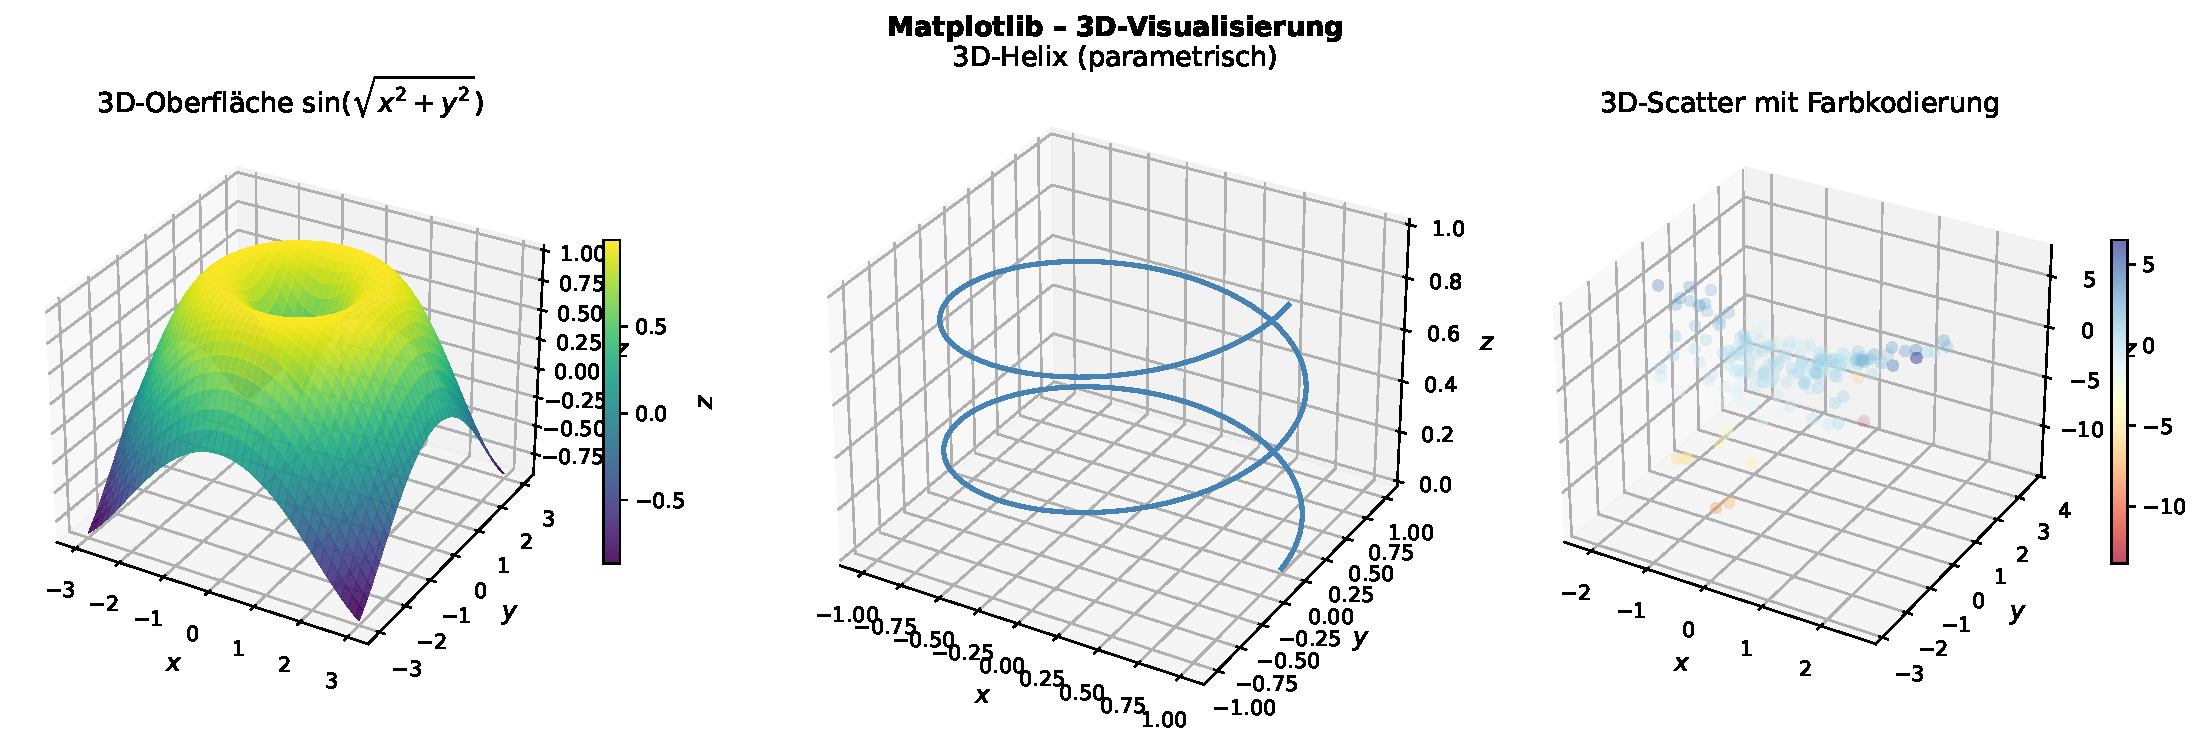
\includegraphics[width=0.7\textwidth]{matplotlib_3d}

  \vspace{1.5cm}
  \begin{tabular}{rl}
    \textbf{Autor:}   & Stephan Epp\\[3pt]
    \textbf{Datum:}   & 18. März 2026\\[3pt]
    \textbf{Sprache:} & Python 3.12\\[3pt]
    \textbf{Schlagwörter:} & Scientific Computing, Data Science,\\
                           & Numerische Mathematik, Datenvisualisierung
  \end{tabular}

  \vfill
  \small\textit{Erstellt mit \LaTeX\ und Python}
\end{titlepage}

\tableofcontents
\listoffigures
\listoftables
\newpage

% ==============================================================
\section{Einleitung}
\label{sec:einleitung}
% ==============================================================

Wissenschaftliches Rechnen erfordert drei wesentliche Fähigkeiten: das
effiziente Verarbeiten numerischer Daten, die Anwendung mathematischer
Algorithmen sowie die überzeugende Visualisierung von Ergebnissen.
Mit dem Aufstieg von Python als \emph{de-facto}-Sprache für Data Science
und wissenschaftliche Forschung hat sich ein Ökosystem um drei zentrale
Bibliotheken herausgebildet, das diese Anforderungen vollständig abdeckt:

\begin{center}
\begin{tabular}{lll}
  \toprule
  \textbf{Bibliothek} & \textbf{Kernaufgabe} & \textbf{Veröffentlicht} \\
  \midrule
  \textcolor{numpyblue}{\textbf{NumPy}} & Numerische Arrays \& lineare Algebra & 2005 \\
  \textcolor{scipygreen}{\textbf{SciPy}} & Wissenschaftliche Algorithmen & 2001 \\
  \textcolor{mplred}{\textbf{Matplotlib}} & 2D/3D-Visualisierung & 2003 \\
  \bottomrule
\end{tabular}
\end{center}

\vspace{0.5em}
Zusammen bilden diese Bibliotheken das sogenannte \emph{Scientific Python
Stack} \cite{virtanen2020scipy, harris2020array, hunter2007matplotlib}.
Sie werden in Peer-Reviewed-Publikationen, Lehrbüchern und industriellen
Anwendungen von Physik über Bioinformatik bis hin zur Finanzwissenschaft
eingesetzt. Allein NumPy wird täglich mehrere Millionen Mal heruntergeladen
und ist in Projekten wie LIGO (Gravitationswellendetektion), NASA-Bildgebung
und der Bildrekonstruktion des Event-Horizon-Teleskops eingesetzt worden
\cite{harris2020array}.

Diese drei Bibliotheken machen eine Software oder eine Anwendung hinsichtlich der mathematischen Beschreibbarkeit vollständig. Und dies muss gezeigt werden. Finde dazu einen Ausdruck in der Mathematik oder in der Regelungstechnik, der mit diesen drei Bibliotheken nicht dargestellt oder nicht beschrieben werden kann. Die Natur hat nicht nur ein Phänomen, welches mathematisch nicht beschrieben werden kann. In der Natur ist Bewegung und diese Bewegung führt aufmerksame Beobachter dahin. Die Bewegung hat seinen Ursprung in der ewigen Energie, welche auch diese Erde gemacht hat und sie erhält in allen ihren Gesetzen. Was dem aufmerksamen Beobachter sofort auffällt, ist, dass die Beschreibung natürlicher Phänomene gar nicht so trivial ist, da diese eher zufällig erscheinen und auftreten. Dabei zeigt sich die Natur dem Beobachter doch auf eine Weise in der zufälligen Art, wie sie dem Beobachter doch intuitiv sehr vertraut ist. Es scheint zu gehen und wieder zu kommen, da zu sein und zu verschwinden. Feuer und Wasser sind dazu die überragenden Beispiele in der Natur. Die geometrische Anordnung bei Tieren ist den Menschen besonders vertraut.

Die Python-Bibliotheken \textbf{NumPy}, \textbf{SciPy} und \textbf{Matplotlib}
bilden das technische Fundament nahezu aller modernen wissenschaftlichen
Arbeiten, die auf Python basieren. Diese Arbeit gibt eine umfassende und
anschauliche Übersicht über die gesamte Ausdrucksstärke dieser drei
Bibliotheken: Vom effizienten numerischen Rechnen mit mehrdimensionalen
Arrays (\emph{NumPy}) über höhere Algorithmen für Gleichungslöser,
Signalverarbeitung, Statistik und wissenschaftliche Spezialfunktionen
(\emph{SciPy}) bis hin zur flexiblen, publikationsreifen
Datenvisualisierung (\emph{Matplotlib}). Anhand zahlreicher kommentierter
Codebeispiele und Abbildungen wird gezeigt, wie diese drei Werkzeuge im
Verbund vollständige wissenschaftliche Arbeitsabläufe ermöglichen –
von der Rohdatenverarbeitung bis zur fertigen Grafik für die Publikation.

In dieser Arbeit werden alle wesentlichen Teilgebiete von NumPy, SciPy und
Matplotlib systematisch vorgestellt, anhand ausführlicher und kommentierter
Python-Codebeispiele illustriert und mit entsprechenden Abbildungen
visualisiert. Am Ende jedes Abschnitts wird der unverzichtbare Wert der
jeweiligen Funktionalität für das wissenschaftliche Arbeiten hervorgehoben.


% ==============================================================
\section{NumPy – Das Fundament des Scientific Computing}
\label{sec:numpy}
% ==============================================================

\subsection{Geschichte und Motivation}
\label{subsec:numpy-history}

Vor NumPy war numerisches Rechnen in Python entweder sehr langsam (via
reine Python-Listen) oder erforderte aufwändige C-Erweiterungen.
\emph{Travis Oliphant} konsolidierte 2005 die Projekte \texttt{Numeric}
und \texttt{numarray} zum modernen NumPy \cite{oliphant2006guide}.
Der Kern von NumPy – das N-dimensionale Array \texttt{ndarray} – ist in
C implementiert und ermöglicht vektorisierte Operationen, die um den
Faktor 100--1000 schneller sind als äquivalenter reiner Python-Code
\cite{harris2020array}.

\subsection{Das ndarray: Kernkonzept}
\label{subsec:numpy-ndarray}

Das zentrale Objekt von NumPy ist das \texttt{ndarray}. Es ist
charakterisiert durch:

\begin{itemize}
  \item \textbf{Form (\texttt{shape})}: Tupel der Dimensionen, z.\,B.\ $(3, 4, 5)$ für ein 3D-Array.
  \item \textbf{Datentyp (\texttt{dtype})}: Homogener Typ aller Elemente (\texttt{float64}, \texttt{int32}, \texttt{complex128}, \ldots).
  \item \textbf{Stride}: Schrittweiten im Speicher, die Ansichten (Views) ohne Kopie ermöglichen.
\end{itemize}

\begin{lstlisting}[caption={Erstellen und Inspizieren von NumPy-Arrays}]
import numpy as np

# 1D-Array aus Python-Liste
a = np.array([1.0, 2.0, 3.0, 4.0])
print(a.shape, a.dtype)   # (4,) float64

# 2D-Array (Matrix)
B = np.array([[1, 2, 3],
              [4, 5, 6]], dtype=np.float64)
print(B.shape)            # (2, 3)

# Spezielle Arrays
zeros = np.zeros((3, 4))           # Nullmatrix
ones  = np.ones((2, 2, 2))         # Einsen-Array
eye   = np.eye(5)                  # Einheitsmatrix
arange = np.arange(0, 10, 0.5)    # Schrittweitenarray
linspace = np.linspace(0, 1, 101) # 101 aequidistante Punkte

# Datentypen-Konversion
c = B.astype(np.complex128)
\end{lstlisting}

\subsection{Vektorisierung und Broadcasting}
\label{subsec:numpy-broadcast}

Broadcasting ist eines der mächtigsten Konzepte von NumPy: Operationen
auf Arrays unterschiedlicher (aber kompatibler) Formen werden automatisch
auf alle Elemente ausgedehnt, ohne unnötige Datenkopien zu erstellen
\cite{vanderplas2016python}.

\begin{lstlisting}[caption={Broadcasting: Elementweise Operationen}]
# Alle 5 Frequenzen auf einmal berechnen (Broadcasting)
x     = np.linspace(0, 2*np.pi, 1000)          # (1000,)
freqs = np.array([1, 2, 3, 4, 5])[:, np.newaxis] # (5, 1)
result = np.sin(freqs * x)                       # (5, 1000)
# Keine Schleife noetig!
\end{lstlisting}

Abbildung~\ref{fig:numpy_overview} (links) zeigt das Ergebnis: Fünf
Sinusschwingungen unterschiedlicher Frequenz, berechnet durch eine
einzige Broadcasting-Operation.

\begin{figure}[H]
  \centering
  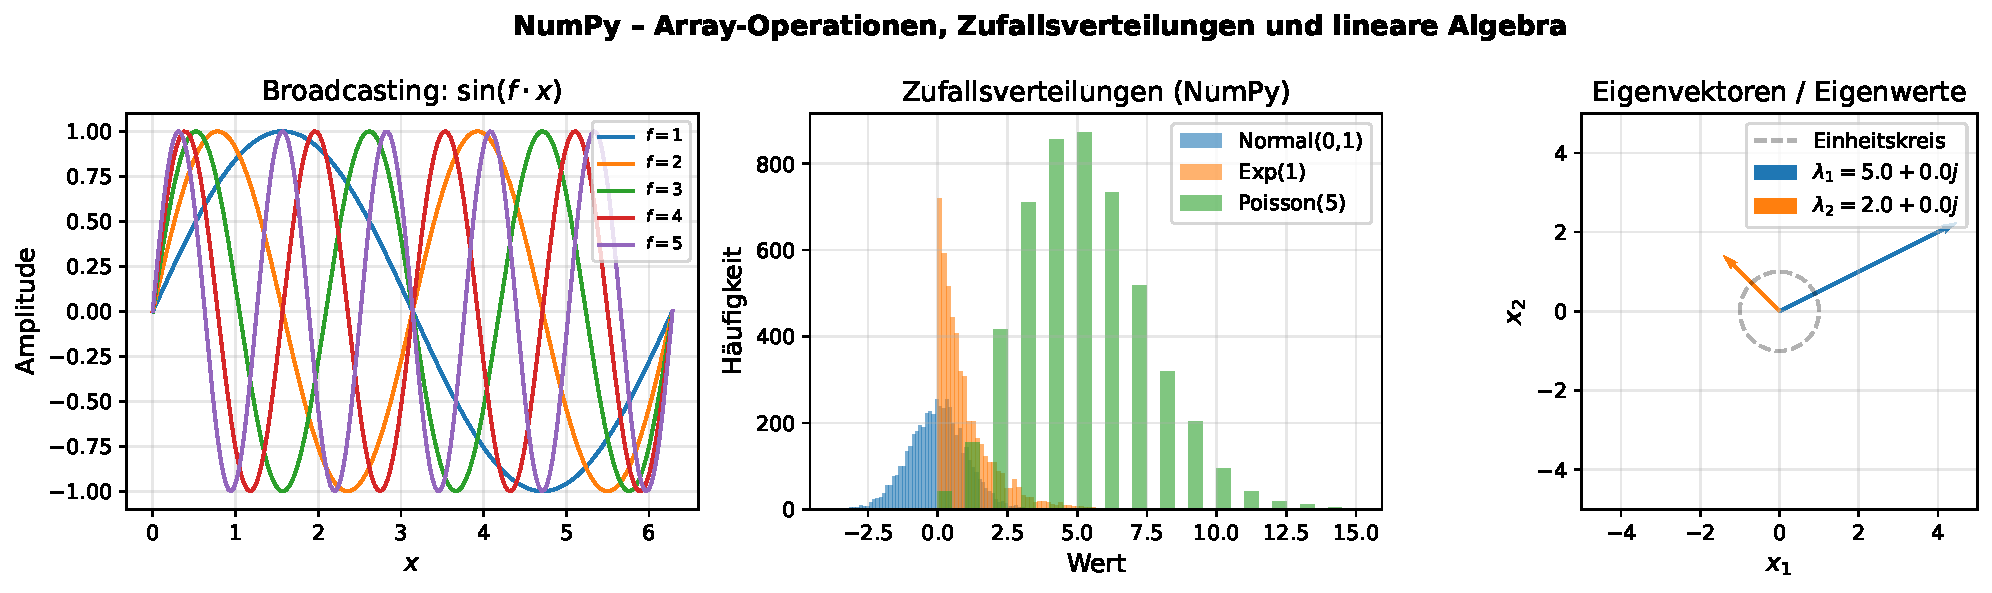
\includegraphics[width=\textwidth]{numpy_overview}
  \caption{NumPy-Ãœbersicht: Broadcasting (links), Zufallsverteilungen (Mitte),
           Eigenvektoren/-werte (rechts).}
  \label{fig:numpy_overview}
\end{figure}

\subsection{Mathematische Universalfunktionen (ufuncs)}
\label{subsec:numpy-ufuncs}

NumPy stellt über 60 \emph{Universal Functions} (ufuncs) bereit, die
elementweise auf Arrays wirken, Broadcasting unterstützen und optionale
Output-Arrays für speichereffizientes Rechnen akzeptieren:

\begin{lstlisting}[caption={Ausgewaehlte NumPy-ufuncs}]
x = np.linspace(-3, 3, 1000)

# Trigonometrisch
y1 = np.sin(x);   y2 = np.cos(x);  y3 = np.tan(x)

# Exponentiell und logarithmisch
y4 = np.exp(x);   y5 = np.log(np.abs(x))
y6 = np.log2(np.abs(x));  y7 = np.log10(np.abs(x))

# Hyperbolisch
y8 = np.sinh(x);  y9 = np.cosh(x)

# Rundung / Vergleich
y10 = np.floor(x)
y11 = np.maximum(x, 0)  # ReLU-Aktivierungsfunktion

# Reduktionfunktionen
print(f"Summe: {x.sum():.4f}, Mittelwert: {x.mean():.4f}")
print(f"Std:   {x.std():.4f}, Varianz:    {x.var():.4f}")
print(f"Min:   {x.min():.4f}, Max:        {x.max():.4f}")
print(f"Kumulative Summe (letzter Wert): {np.cumsum(x)[-1]:.4f}")
\end{lstlisting}

\subsection{Lineare Algebra mit NumPy}
\label{subsec:numpy-linalg}

Das Untermodul \texttt{numpy.linalg} implementiert alle grundlegenden
Operationen der linearen Algebra:

\begin{lstlisting}[caption={Lineare Algebra: Eigenwerte, Matrixoperationen}]
import numpy as np

A = np.array([[4, 2, 0],
              [1, 3, 1],
              [0, 2, 5]], dtype=float)

# Determinante
det_A = np.linalg.det(A)   # ~44.0

# Inverse
A_inv = np.linalg.inv(A)

# Eigenwertzerlegung
eigenvalues, eigenvectors = np.linalg.eig(A)
print("Eigenwerte:", eigenvalues)   # [5.73, 4.41, 1.86]

# LU (via numpy): als QR
Q, R = np.linalg.qr(A)  # A = Q @ R

# Gleichungssystem A x = b
b = np.array([1.0, 2.0, 3.0])
x = np.linalg.solve(A, b)
print("Loesung:", x)

# Konditionszahl
kappa = np.linalg.cond(A)

# Singulärwertzerlegung (SVD)
U, sigma, Vt = np.linalg.svd(A)
A_reconstruct = U @ np.diag(sigma) @ Vt   # = A
\end{lstlisting}

Abbildung~\ref{fig:numpy_overview} (rechts) visualisiert die Eigenvektoren
einer $(2\times2)$-Matrix: Die Vektoren zeigen in die Richtungen, die durch
die lineare Abbildung nicht gedreht, sondern nur skaliert werden.

\subsection{Zufallszahlengenerierung}
\label{subsec:numpy-random}

NumPy bietet einen modernen und reproduzierbaren Zufallszahlengenerator
(\texttt{numpy.random.\allowbreak{}default\_rng}) auf Basis des PCG64-Algorithmus:

\begin{lstlisting}[caption={Zufallsverteilungen mit NumPy}]
rng = np.random.default_rng(seed=42)  # reproduzierbar

# Normalverteilung N(mu, sigma)
normal_data = rng.normal(loc=0, scale=1, size=(1000, 3))

# Gleichverteilung [a, b)
uniform_data = rng.uniform(low=0, high=1, size=5000)

# Ganzzahlige Gleichverteilung
dice = rng.integers(1, 7, size=10000)   # Würfelsimulation

# Poisson-Prozess
poisson = rng.poisson(lam=5, size=10000)

# Multivariate Gauss-Verteilung
mean = np.array([0, 0])
cov  = np.array([[1, 0.8], [0.8, 1]])
mvn  = rng.multivariate_normal(mean, cov, size=2000)

# Mischen / Stichproben
shuffled = rng.permutation(np.arange(100))
sample   = rng.choice(np.arange(50), size=10, replace=False)
\end{lstlisting}

Abbildung~\ref{fig:numpy_overview} (Mitte) vergleicht Histogramme der Normal-,
Exponential- und Poisson-Verteilung für je 5\,000 Realisierungen.

\subsection{Fourier-Transformation mit NumPy}
\label{subsec:numpy-fft}

Fourier-Transformationen sind fundamental in der Signal- und Bildverarbeitung.
NumPy enthält eine vollständige FFT-Implementierung:

\begin{lstlisting}[caption={FFT mit NumPy}]
fs = 1000.0                              # Abtastrate [Hz]
t  = np.linspace(0, 1, int(fs))         # Zeitvektor [s]

# Zusammengesetztes Signal
sig = (np.sin(2*np.pi*50*t)
      + 0.5*np.sin(2*np.pi*120*t)
      + 0.3*rng.normal(size=len(t)))

# FFT
freqs_fft = np.fft.rfftfreq(len(t), 1/fs)  # einseitiges Spektrum
spectrum  = np.abs(np.fft.rfft(sig))        # Betragsspektrum

# Inverse FFT
sig_reconstructed = np.fft.irfft(np.fft.rfft(sig))
\end{lstlisting}

Abbildung~\ref{fig:numpy_fft_poly} zeigt den Zeitverlauf (links) und das
zugehörige Frequenzspektrum (Mitte), in dem die Peaks bei 50\,Hz und
120\,Hz klar erkennbar sind.

\begin{figure}[H]
  \centering
  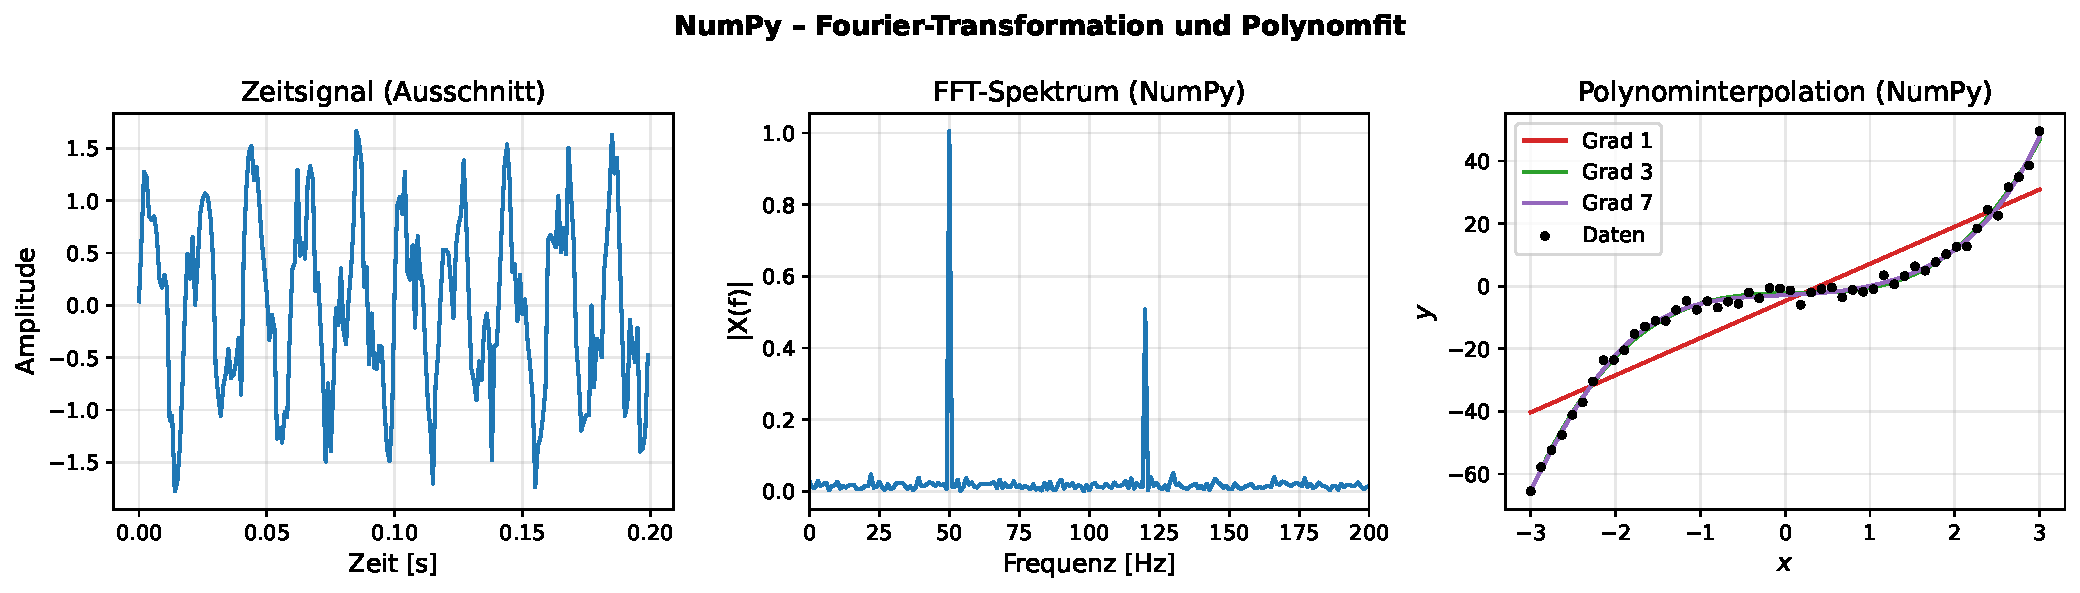
\includegraphics[width=\textwidth]{numpy_fft_poly}
  \caption{NumPy FFT: Zeitsignal (links), Betragsspektrum (Mitte),
           Polynomfit verschiedener Grade (rechts).}
  \label{fig:numpy_fft_poly}
\end{figure}

\subsection{Polynome und Kurvenanpassung}
\label{subsec:numpy-polyfit}

\texttt{numpy.polyfit} und \texttt{numpy.poly1d} ermöglichen einfache
Polynominterpolation und -regression:

\begin{lstlisting}[caption={Polynomfit mit NumPy}]
x_data = np.linspace(-3, 3, 50)
y_data = 2*x_data**3 - x_data**2 + 0.5*x_data - 1 + rng.normal(0, 2, 50)

for degree in [1, 3, 7]:
    coeffs = np.polyfit(x_data, y_data, degree)
    poly   = np.poly1d(coeffs)               # auswertbares Polynom
    x_fit  = np.linspace(-3, 3, 300)
    y_fit  = poly(x_fit)                     # Auswertung
    # Bewertungsmassstab:
    residuals = y_data - poly(x_data)
    r_squared = 1 - np.var(residuals)/np.var(y_data)
    print(f"Grad {degree}: R^2 = {r_squared:.4f}")
\end{lstlisting}

Abbildung~\ref{fig:numpy_fft_poly} (rechts) illustriert die Ãœberanpassung
(\emph{Overfitting}) bei Grad~7 im Vergleich zum theoretisch korrekten
Grad-3-Polynom.

\subsection{Einzigartiger Wert von NumPy}

NumPy transformiert Python von einer interpretierten Skriptsprache zu
einem leistungsfähigen numerischen Rechenwerkzeug. Durch Vektorisierung,
Broadcasting und die enge Integration mit optimierten BLAS/LAPACK-Routinen
werden Berechnungen, die in reinem Python Minuten benötigen würden, in
Millisekunden ausgeführt. Kein anderes Python-Konstrukt bietet diese
Kombination aus \emph{Ausdrucksstärke}, \emph{Effizienz} und
\emph{Portabilität}.

% ==============================================================
\section{SciPy – Höhere Algorithmen für die Wissenschaft}
\label{sec:scipy}
% ==============================================================

\subsection{Ãœberblick und Architektur}
\label{subsec:scipy-overview}

SciPy baut auf NumPy auf und ergänzt es durch über 500 hochspezialisierte
Funktionen, die in thematischen Submodulen organisiert sind
\cite{virtanen2020scipy}:

\begin{center}
\begin{longtable}{p{4.5cm}p{3.5cm}p{5.5cm}}
  \toprule
  \textbf{Submodul} & \textbf{Bereich} & \textbf{Wesentliche Inhalte}\\
  \midrule
  \endhead
  \texttt{scipy.linalg}     & Lineare Algebra   & LU, QR, SVD, Cholesky, Schur, Lyapunov \\
  \texttt{scipy.optimize}   & Optimierung       & Gradientenverfahren, BFGS, Evolutionsstrategien, curve\_fit \\
  \texttt{scipy.integrate}  & Integration/DGL   & quad, dblquad, solve\_ivp (RK45, DOP853, BDF) \\
  \texttt{scipy.signal}     & Signalverarbeitung & Filter, Spektrogramme, Faltung, Wavelets \\
  \texttt{scipy.stats}      & Statistik         & Verteilungen, Hypothesentests, KDE \\
  \texttt{scipy.interpolate}& Interpolation     & Splines, RBF, Barycenterinterpolation \\
  \texttt{scipy.fft}        & Fourier-Analyse   & FFT, DCT, DST (schneller als NumPy-FFT) \\
  \texttt{scipy.sparse}     & Dünnbesetzte Matrizen & CSR, CSC, Eigenwertsolver \\
  \texttt{scipy.spatial}    & Geometrie         & KD-Tree, Voronoi, Delaunay, Konvexhülle \\
  \texttt{scipy.special}    & Spezialfunktionen & Bessel, Gamma, Legendre, elliptische Integrale \\
  \texttt{scipy.ndimage}    & Bildverarbeitung  & Gauss-Glättung, Morphologie, Messungen \\
  \texttt{scipy.io}         & Datei-I/O         & MATLAB-, WAV-, ARFF-Dateien lesen/schreiben \\
  \bottomrule
  \caption{SciPy-Submodule und ihre Inhalte \cite{virtanen2020scipy}.}
  \label{tab:scipy_modules}
\end{longtable}
\end{center}

\subsection{Lineare Algebra mit SciPy}
\label{subsec:scipy-linalg}

\texttt{scipy.linalg} bietet gegenüber \texttt{numpy.linalg} erweiterte
Zerlegungsverfahren und ist für viele Matrixoperationen schneller, da
es gezielt auf LAPACK zugreift:

\begin{lstlisting}[caption={Fortgeschrittene lineare Algebra mit SciPy}]
from scipy import linalg
import numpy as np

rng = np.random.default_rng(42)
A = rng.normal(size=(6, 6))

# Singulaerwertzerlegung A = U @ diag(sigma) @ V^T
U, sigma, Vt = linalg.svd(A)
print("Singulaerwerte:", np.round(sigma, 3))

# LU-Zerlegung: A = P @ L @ U
P, L, U = linalg.lu(A)

# QR-Zerlegung mit Column-Pivoting
Q, R, P_qr = linalg.qr(A, pivoting=True)

# Cholesky (positiv definit erforderlich)
AA = A @ A.T + 5*np.eye(6)          # definitiv positiv definit
L_chol = linalg.cholesky(AA, lower=True)

# Schur-Zerlegung A = Z @ T @ Z^H
T_schur, Z = linalg.schur(A)

# Lineare Gleichungssysteme (schneller als numpy)
b = rng.normal(size=6)
x_sol = linalg.solve(A, b)

# Pseudo-Inverse (Least Squares)
A_rect = rng.normal(size=(8, 4))  # ueberbestimmtes System
b_rect = rng.normal(size=8)
x_ls   = linalg.lstsq(A_rect, b_rect)[0]
\end{lstlisting}

\begin{figure}[H]
  \centering
  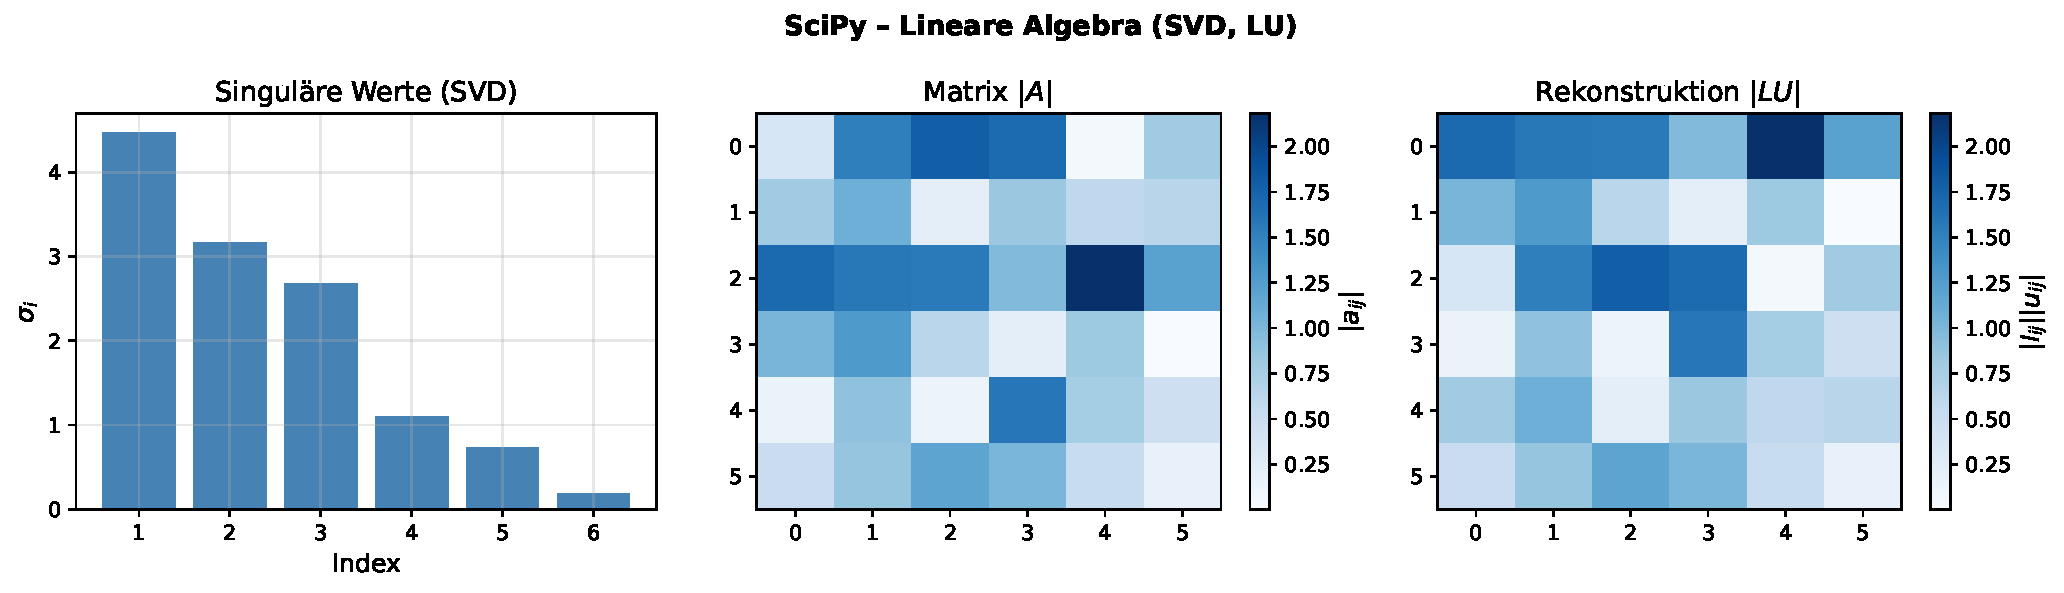
\includegraphics[width=\textwidth]{scipy_linalg}
  \caption{SciPy lineare Algebra: Singuläre Werte (links),
           Originalmatrix $|A|$ (Mitte), Rekonstruktion $|LU|$ (rechts).}
  \label{fig:scipy_linalg}
\end{figure}

\subsection{Numerische Optimierung}
\label{subsec:scipy-optimize}

\texttt{scipy.optimize} ist ein vollständiges Optimierungspaket für
ein- und mehrdimensionale Probleme mit und ohne Nebenbedingungen:

\begin{lstlisting}[caption={Optimierung mit SciPy: BFGS, Trust-Region und Global}]
from scipy import optimize
import numpy as np

# --- 1. Unbeschraenkte Optimierung (L-BFGS-B) ---
def rosenbrock(xy):
    x, y = xy
    return (1 - x)**2 + 100*(y - x**2)**2

result = optimize.minimize(
    rosenbrock, x0=[-1.5, 0.5],
    method='L-BFGS-B',
    options={'ftol': 1e-12, 'maxiter': 2000}
)
print(f"Minimum: {result.x}, f = {result.fun:.2e}")
# Minimum: [1. 1.], f = 1.23e-20

# --- 2. Beschraenkte Optimierung (SLSQP) ---
def objective(x):
    return -x[0] * x[1] * x[2]   # Volumen maximieren

constraints = [{'type': 'eq', 'fun': lambda x: 2*(x[0]*x[1]+x[1]*x[2]+x[0]*x[2]) - 1}]
bounds = [(0.01, None)]*3

res_constrained = optimize.minimize(
    objective, [0.3, 0.3, 0.3],
    method='SLSQP', bounds=bounds, constraints=constraints
)

# --- 3. Differentielle Evolution (Global) ---
result_de = optimize.differential_evolution(
    rosenbrock, bounds=[(-2, 2), (-1, 3)], seed=42, maxiter=1000
)

# --- 4. Curve Fitting ---
def model(x, a, b, c):
    return a * np.exp(-b*x) * np.cos(c*x)

xdata = np.linspace(0, 4*np.pi, 80)
ydata = model(xdata, 3, 0.3, 2) + 0.2*np.random.default_rng(5).normal(size=80)
popt, pcov = optimize.curve_fit(model, xdata, ydata, p0=[2, 0.5, 1.5])
perr = np.sqrt(np.diag(pcov))   # Parameterunsicherheiten
print(f"a = {popt[0]:.3f} +- {perr[0]:.3f}")
\end{lstlisting}

\begin{figure}[H]
  \centering
  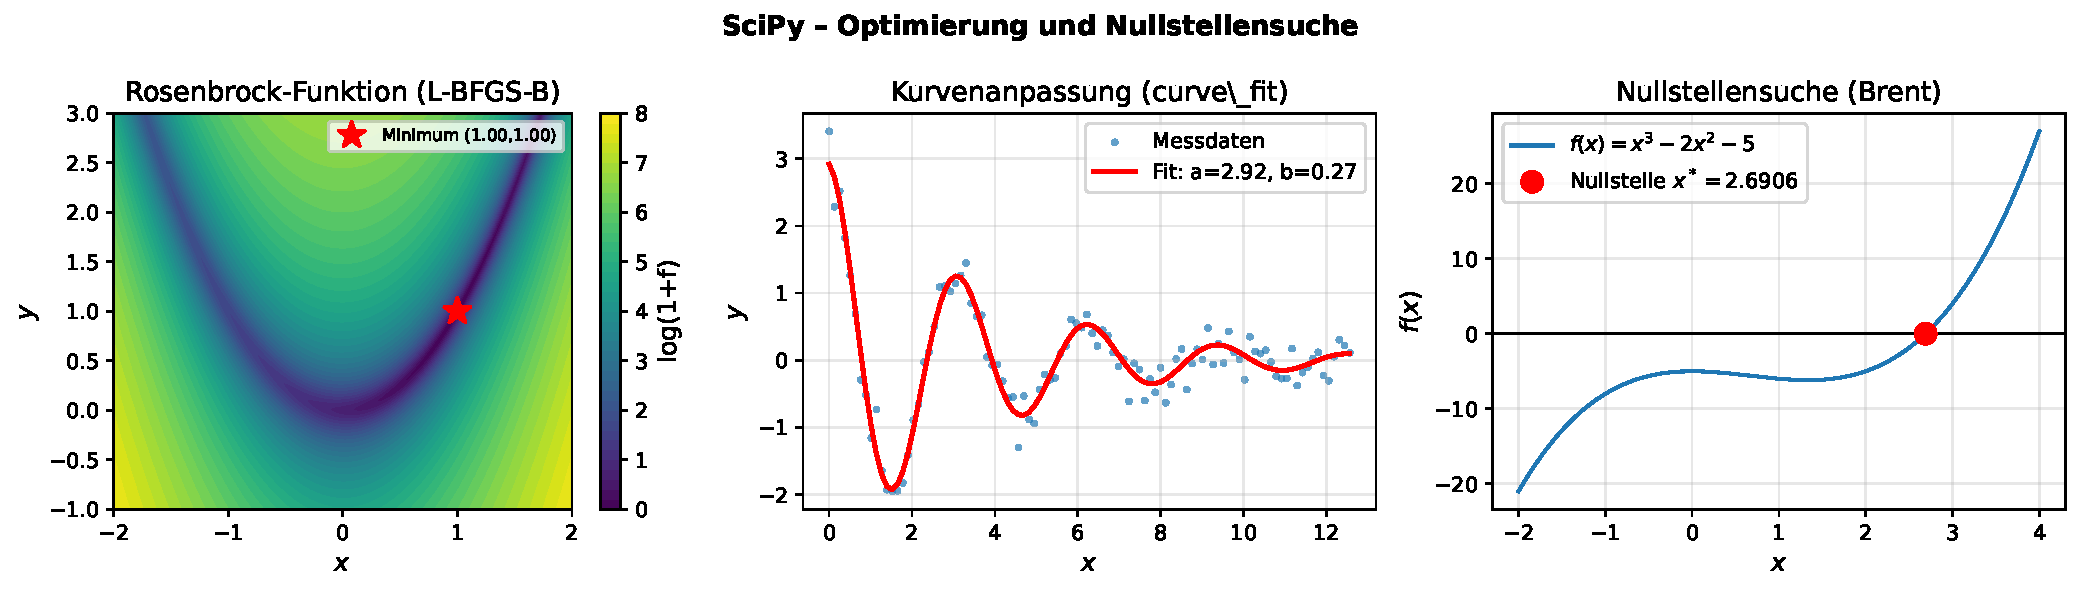
\includegraphics[width=\textwidth]{scipy_optimize}
  \caption{SciPy Optimierung: Rosenbrock-Funktion mit L-BFGS-B-Minimum (links),
           Kurvenanpassung (Mitte), Nullstellensuche (rechts).}
  \label{fig:scipy_optimize}
\end{figure}

\subsection{Numerische Integration und Differentialgleichungen}
\label{subsec:scipy-integrate}

\texttt{scipy.integrate} löst sowohl bestimmte Integrale als auch
gewöhnliche Differentialgleichungssysteme:

\begin{lstlisting}[caption={Integration und DGL-Loesung mit SciPy}]
from scipy import integrate
import numpy as np

# --- Bestimmtes Integral ---
def f(x):
    return np.exp(-x**2) * np.cos(4*x)

value, error = integrate.quad(f, -np.inf, np.inf)
print(f"Integral = {value:.6f}, Fehler = {error:.2e}")

# --- Doppelintegral ---
def g(x, y):
    return np.exp(-x**2 - y**2)

val2d, _ = integrate.dblquad(g, -3, 3, -3, 3)

# --- Lotka-Volterra DGL-System ---
def lotka_volterra(t, y, alpha, beta, delta, gamma):
    x, yy = y
    dxdt = alpha*x   - beta*x*yy
    dydt = delta*x*yy - gamma*yy
    return [dxdt, dydt]

sol = integrate.solve_ivp(
    lotka_volterra, t_span=(0, 30), y0=[10, 5],
    args=(1.5, 0.1, 0.075, 1.5),
    method='RK45', rtol=1e-8, atol=1e-10,
    t_eval=np.linspace(0, 30, 2000)
)

# --- Steifes DGL-System (Chemie) ---
def robertson(t, y):
    k1, k2, k3 = 0.04, 3e7, 1e4
    dy1 = -k1*y[0] + k3*y[1]*y[2]
    dy2 =  k1*y[0] - k2*y[1]**2 - k3*y[1]*y[2]
    dy3 =  k2*y[1]**2
    return [dy1, dy2, dy3]

sol_stiff = integrate.solve_ivp(
    robertson, (0, 1e11), [1, 0, 0],
    method='BDF',                     # implizit, fuer steife Systeme
    rtol=1e-6, atol=[1e-6, 1e-10, 1e-6]
)
\end{lstlisting}

\begin{figure}[H]
  \centering
  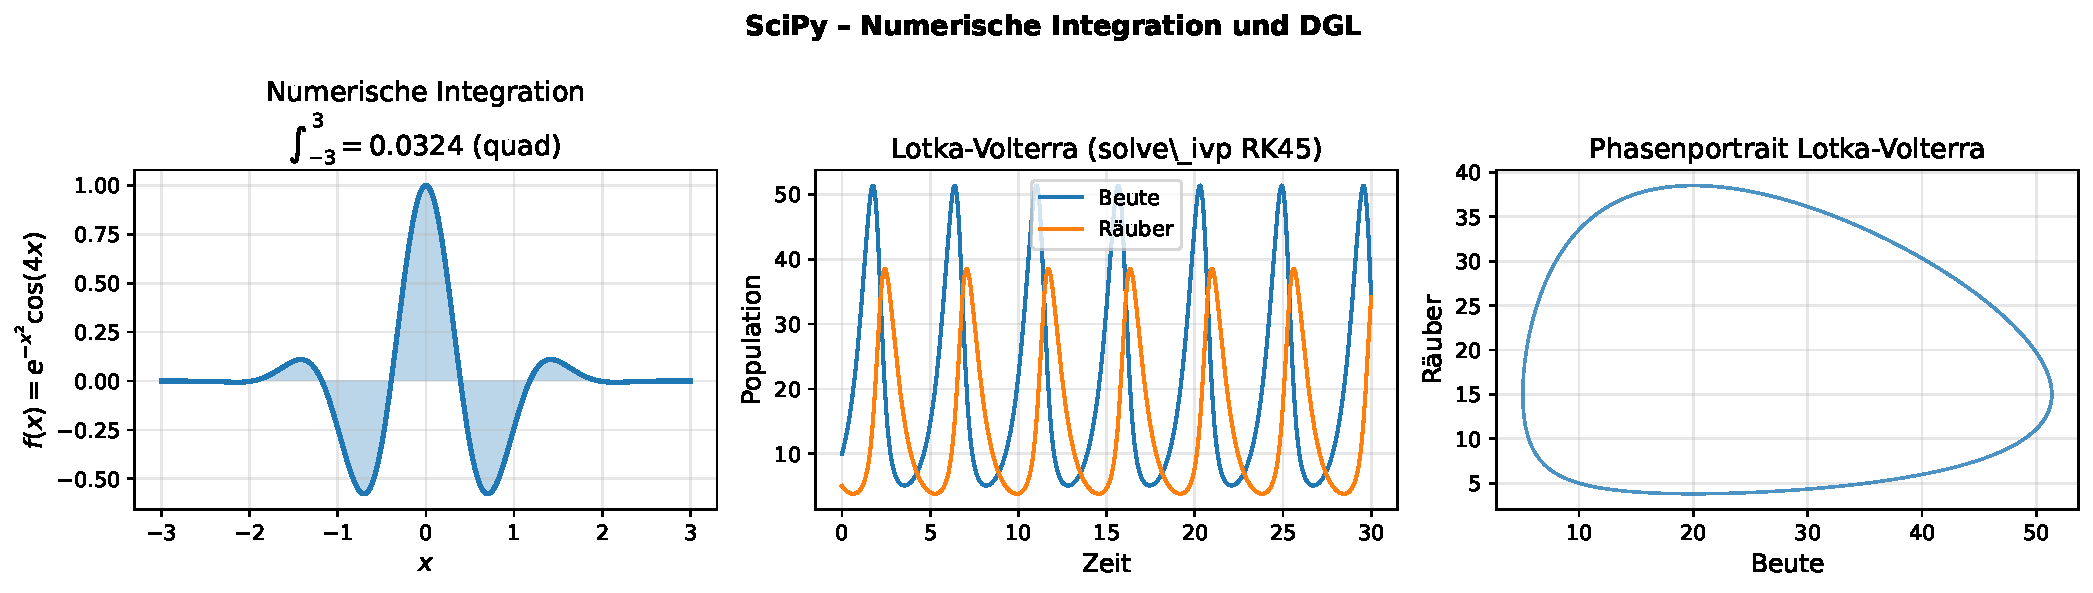
\includegraphics[width=\textwidth]{scipy_integrate}
  \caption{SciPy Integration: Numerisches Integral (links), Lotka-Volterra-
           Populationsdynamik (Mitte), Phasenportrait (rechts).}
  \label{fig:scipy_integrate}
\end{figure}

Das Lotka-Volterra-Modell \cite{lotka1925elements} beschreibt die
Wechselwirkung zwischen Räuber und Beute:
\begin{align}
  \frac{\mathrm{d}x}{\mathrm{d}t} &= \alpha x - \beta x y,\\
  \frac{\mathrm{d}y}{\mathrm{d}t} &= \delta x y - \gamma y,
\end{align}
wobei $x$ die Beutepopulation und $y$ die Räuberpopulation bezeichnet.
Die periodischen Lösungsorbits im Phasenraum (Abb.~\ref{fig:scipy_integrate} rechts)
sind ein klassisches Beispiel nichtlinearer Dynamik.

\subsection{Signalverarbeitung}
\label{subsec:scipy-signal}

\texttt{scipy.signal} bietet eine vollständige Signalverarbeitungs-Toolbox:

\begin{lstlisting}[caption={Signalverarbeitung mit SciPy}]
from scipy import signal
import numpy as np

fs = 500.0
t  = np.linspace(0, 2, int(2*fs))

# Chirp-Signal (frequenzmoduliert)
chirp_sig = signal.chirp(t, f0=1, f1=100, t1=2, method='linear')

# --- IIR-Filter Design ---
# Butterworth-Tiefpass, 5. Ordnung, Grenzfrequenz 40 Hz
b_lp, a_lp = signal.butter(5, 40, btype='lowpass', fs=fs)
y_lp = signal.filtfilt(b_lp, a_lp, chirp_sig)  # Nullphasenfilterer

# Bandpassfilter
b_bp, a_bp = signal.butter(4, [20, 80], btype='bandpass', fs=fs)

# Chebyshev-I (steilere Flanken, Welligkeit im Durchlassbereich)
b_ch, a_ch = signal.cheby1(5, 1, 40, btype='low', fs=fs)  # 1 dB Ripple

# FIR-Filter (windowing-Methode)
n_fir = 101
b_fir = signal.firwin(n_fir, cutoff=40, window='hamming', fs=fs)
y_fir = signal.convolve(chirp_sig, b_fir, mode='same')

# Spektrogramm
f_sg, t_sg, Sxx = signal.spectrogram(
    chirp_sig, fs=fs, nperseg=128, noverlap=64
)

# Welch-Leistungsdichtespektrum
f_welch, Pxx = signal.welch(chirp_sig, fs=fs, nperseg=256)

# Kreuzleistungsspektrum
f_csd, Cxy = signal.csd(chirp_sig, y_lp, fs=fs, nperseg=256)

# Coherenz
f_coh, Coh = signal.coherence(chirp_sig, y_lp, fs=fs, nperseg=256)
\end{lstlisting}

\begin{figure}[H]
  \centering
  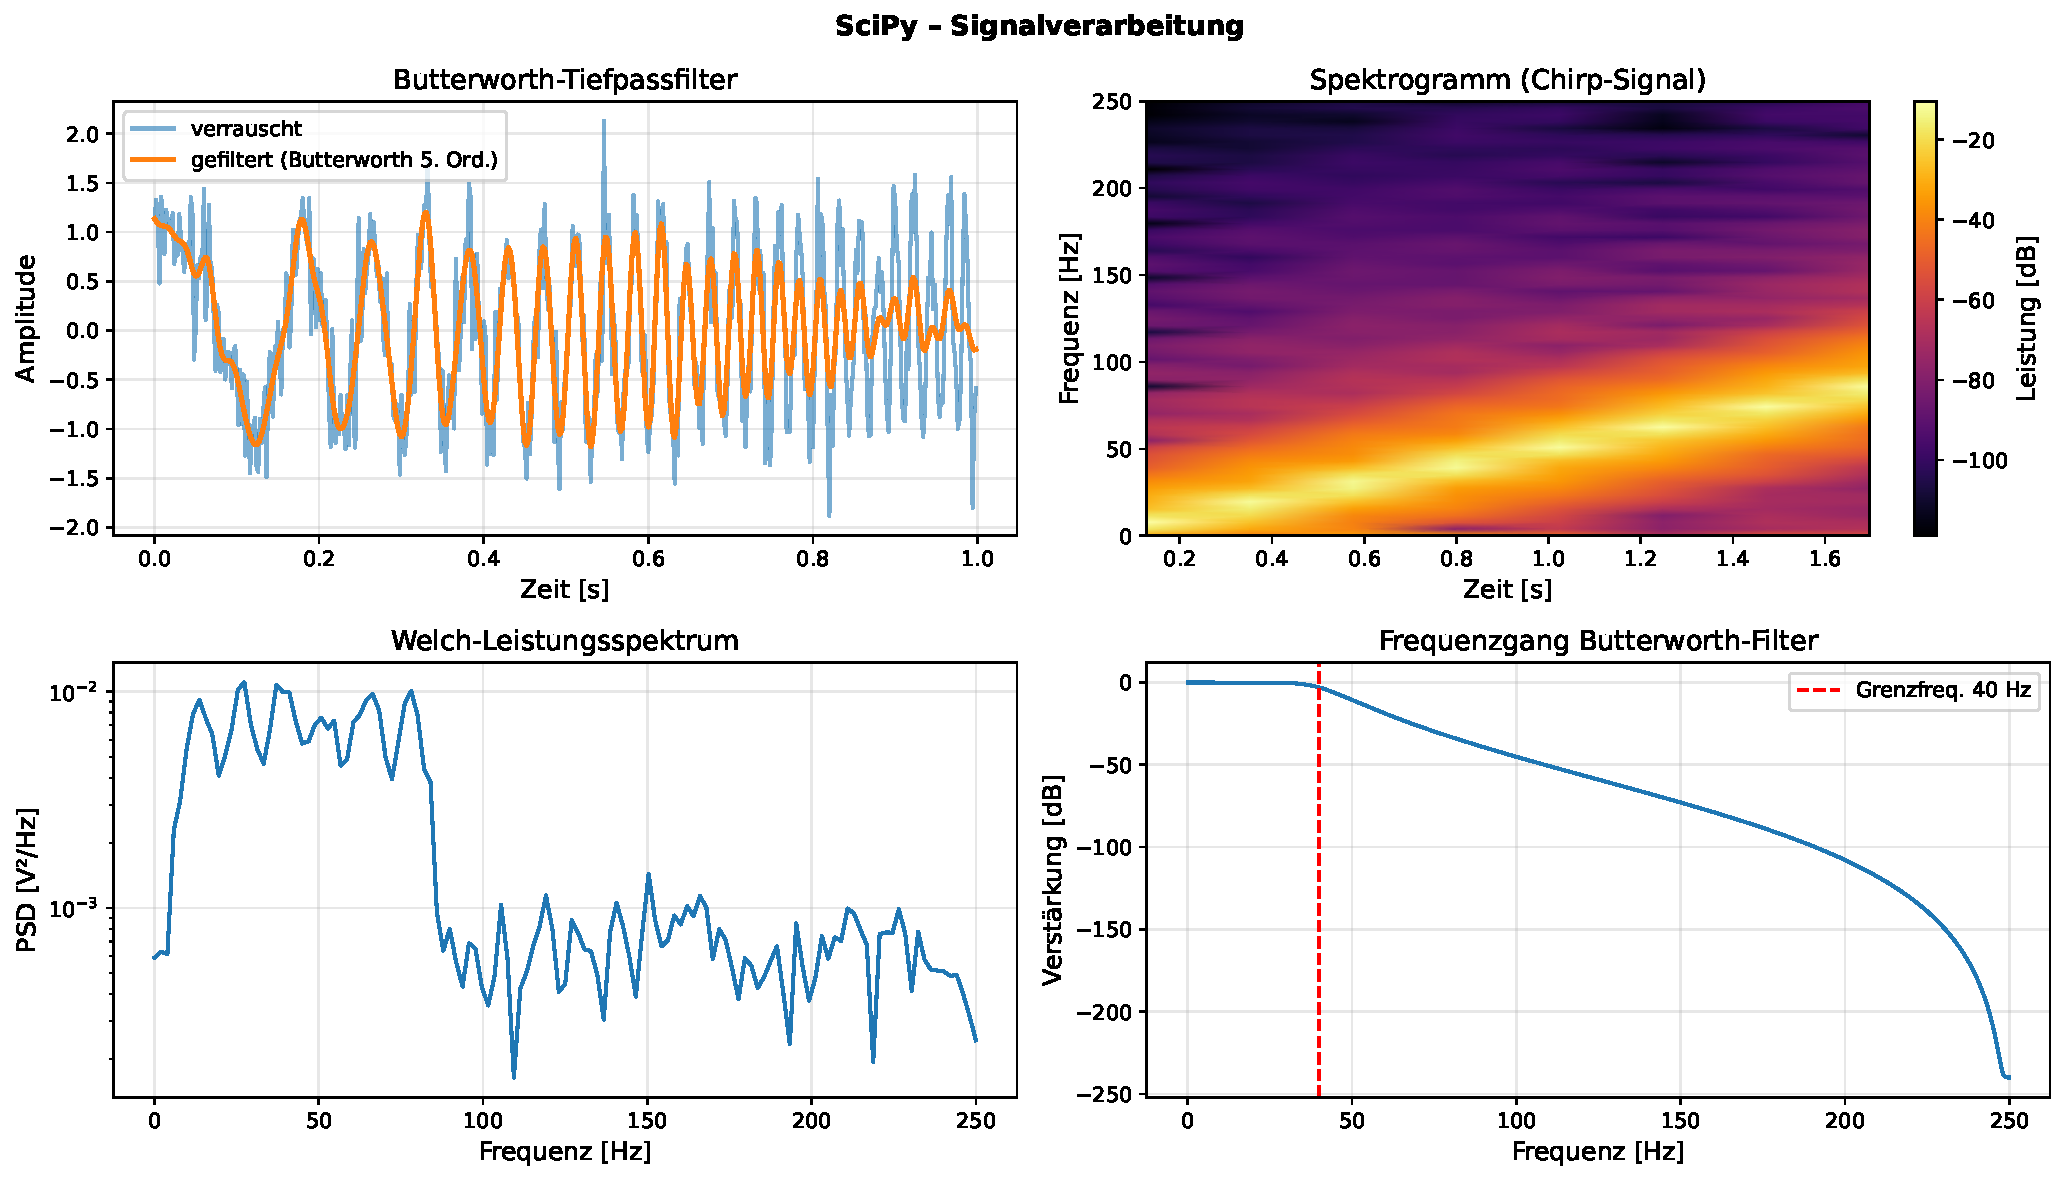
\includegraphics[width=\textwidth]{scipy_signal}
  \caption{SciPy Signalverarbeitung: Butterworth-Tiefpass (oben links),
           Spektrogramm des Chirp-Signals (oben rechts), Welch-PSD
           (unten links), Filterfrequenzgang (unten rechts).}
  \label{fig:scipy_signal}
\end{figure}

\subsection{Wahrscheinlichkeitsstatistik}
\label{subsec:scipy-stats}

\texttt{scipy.stats} enthält über 100 kontinuierliche und diskrete
Wahrscheinlichkeitsverteilungen sowie eine Vielzahl statistischer Tests:

\begin{lstlisting}[caption={Statistische Analysen mit SciPy}]
from scipy import stats
import numpy as np

rng = np.random.default_rng(99)
sample1 = rng.normal(5, 1.5, 200)
sample2 = rng.normal(6, 2.0, 200)

# Lageparameter und Streuung
print(f"Mittelwert: {np.mean(sample1):.3f}")
print(f"Median:     {np.median(sample1):.3f}")
print(f"IQR:        {stats.iqr(sample1):.3f}")
print(f"Schiefe:    {stats.skew(sample1):.3f}")
print(f"Kurtosis:   {stats.kurtosis(sample1):.3f}")

# t-Test (zweiseitig, unabhaengige Stichproben)
t_stat, p_value = stats.ttest_ind(sample1, sample2)
print(f"t-Test: t={t_stat:.3f}, p={p_value:.4f}")

# Wilcoxon-Mann-Whitney-U-Test (nicht-parametrisch)
u_stat, p_mw = stats.mannwhitneyu(sample1, sample2, alternative='two-sided')

# Kolmogorov-Smirnov-Test auf Normalverteilung
ks_stat, p_ks = stats.kstest(sample1, 'norm',
                              args=(np.mean(sample1), np.std(sample1)))

# Shapiro-Wilk-Test
sw_stat, p_sw = stats.shapiro(sample1[:50])  # max 50 Datenpunkte empfohlen

# Pearson-Korrelation
r_pearson, p_pearson = stats.pearsonr(sample1, sample2)

# Spearman-Rangkorrelation
r_spearman, p_spearman = stats.spearmanr(sample1, sample2)

# Kernel-Dichteschaetzung (KDE)
kde = stats.gaussian_kde(sample1, bw_method='scott')
x_eval = np.linspace(0, 12, 400)
pdf_est = kde(x_eval)

# Anpassungstest: beste Verteilung finden
list_dists = [stats.norm, stats.lognorm, stats.gamma, stats.beta]
for dist in list_dists:
    fit_params = dist.fit(sample1)
    ks, p = stats.kstest(sample1, dist.name, args=fit_params)
    print(f"{dist.name}: KS={ks:.4f}, p={p:.4f}")
\end{lstlisting}

\begin{figure}[H]
  \centering
  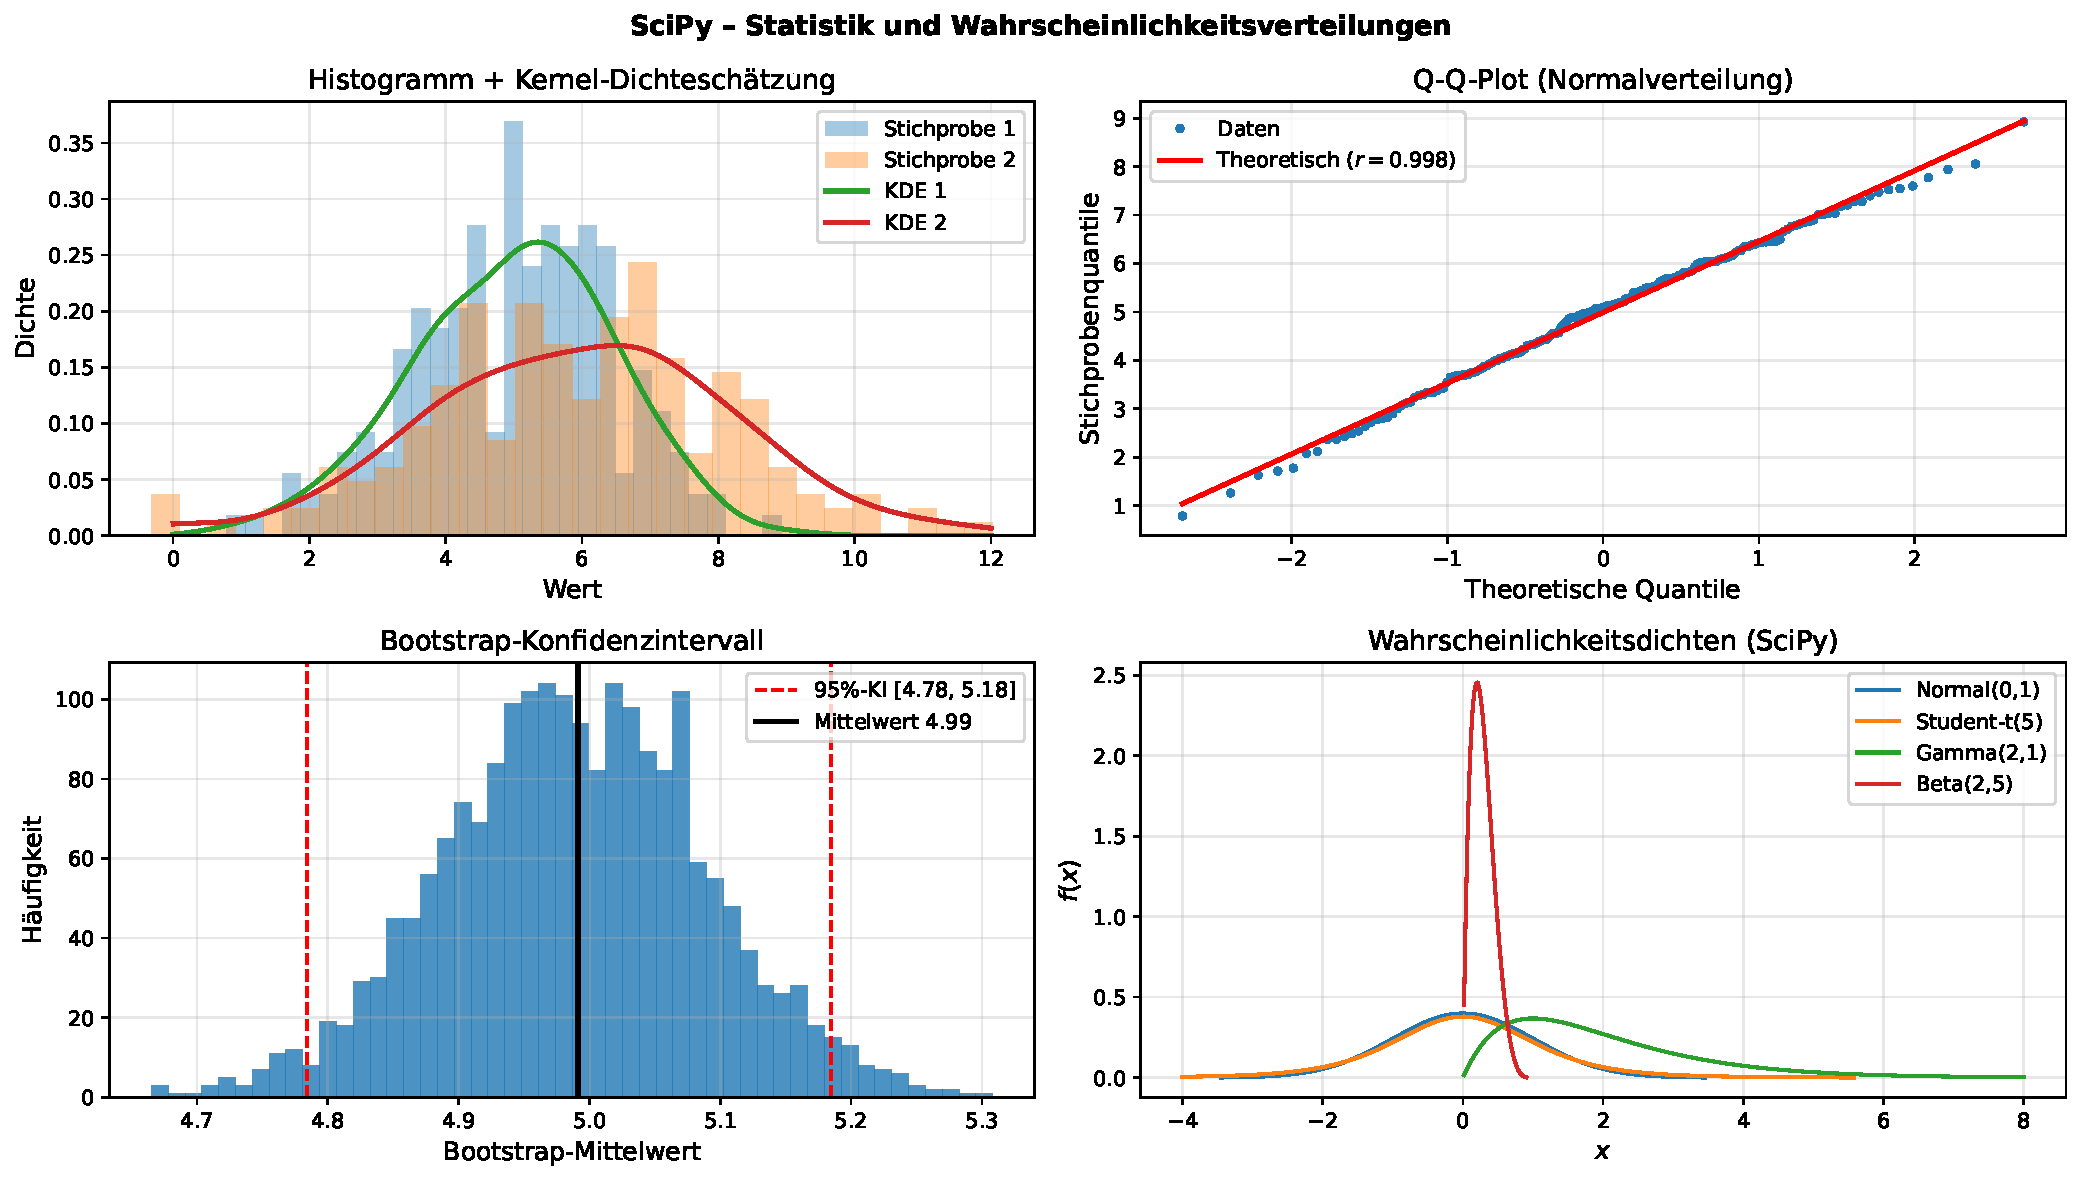
\includegraphics[width=\textwidth]{scipy_stats}
  \caption{SciPy Statistik: KDE und Histogramm (oben links), Q-Q-Plot
           (oben rechts), Bootstrap-Konfidenzintervall (unten links),
           Wahrscheinlichkeitsdichten (unten rechts).}
  \label{fig:scipy_stats}
\end{figure}

\subsection{Interpolation}
\label{subsec:scipy-interp}

\texttt{scipy.interpolate} bietet eine Vielzahl von Interpolationsverfahren
für ein- und mehrdimensionale Daten:

\begin{lstlisting}[caption={Interpolation mit SciPy}]
from scipy import interpolate
import numpy as np

# --- 1D Spline-Interpolation ---
x_pts = np.array([0, 1, 2, 3, 4, 5, 6])
y_pts = np.array([0, 0.8, 0.9, 0.1, -0.8, -1, -0.4])

f_lin   = interpolate.interp1d(x_pts, y_pts, kind='linear')
f_cubic = interpolate.interp1d(x_pts, y_pts, kind='cubic')
f_quad  = interpolate.interp1d(x_pts, y_pts, kind='quadratic')

# PCHIP: erhält Monotonie
f_pchip = interpolate.PchipInterpolator(x_pts, y_pts)

# Baryzentrischer Lagrange-Interpolation
f_bary  = interpolate.BarycentricInterpolator(x_pts, y_pts)

# UnivariateSpline mit Glaettungsparameter
f_us    = interpolate.UnivariateSpline(x_pts, y_pts, s=0.5)

# --- 2D RBF (Radial Basis Function) ---
from scipy.interpolate import RBFInterpolator
rng = np.random.default_rng(5)
xy_pts = rng.uniform(-2, 2, (60, 2))
z_pts  = np.sin(np.pi*xy_pts[:,0]) * np.cos(np.pi*xy_pts[:,1])
rbf = RBFInterpolator(xy_pts, z_pts, kernel='thin_plate_spline')

# Auswertung auf Gitter
xg = np.linspace(-2, 2, 80)
yg = np.linspace(-2, 2, 80)
XG, YG = np.meshgrid(xg, yg)
ZG = rbf(np.column_stack([XG.ravel(), YG.ravel()])).reshape(80, 80)
\end{lstlisting}

\begin{figure}[H]
  \centering
  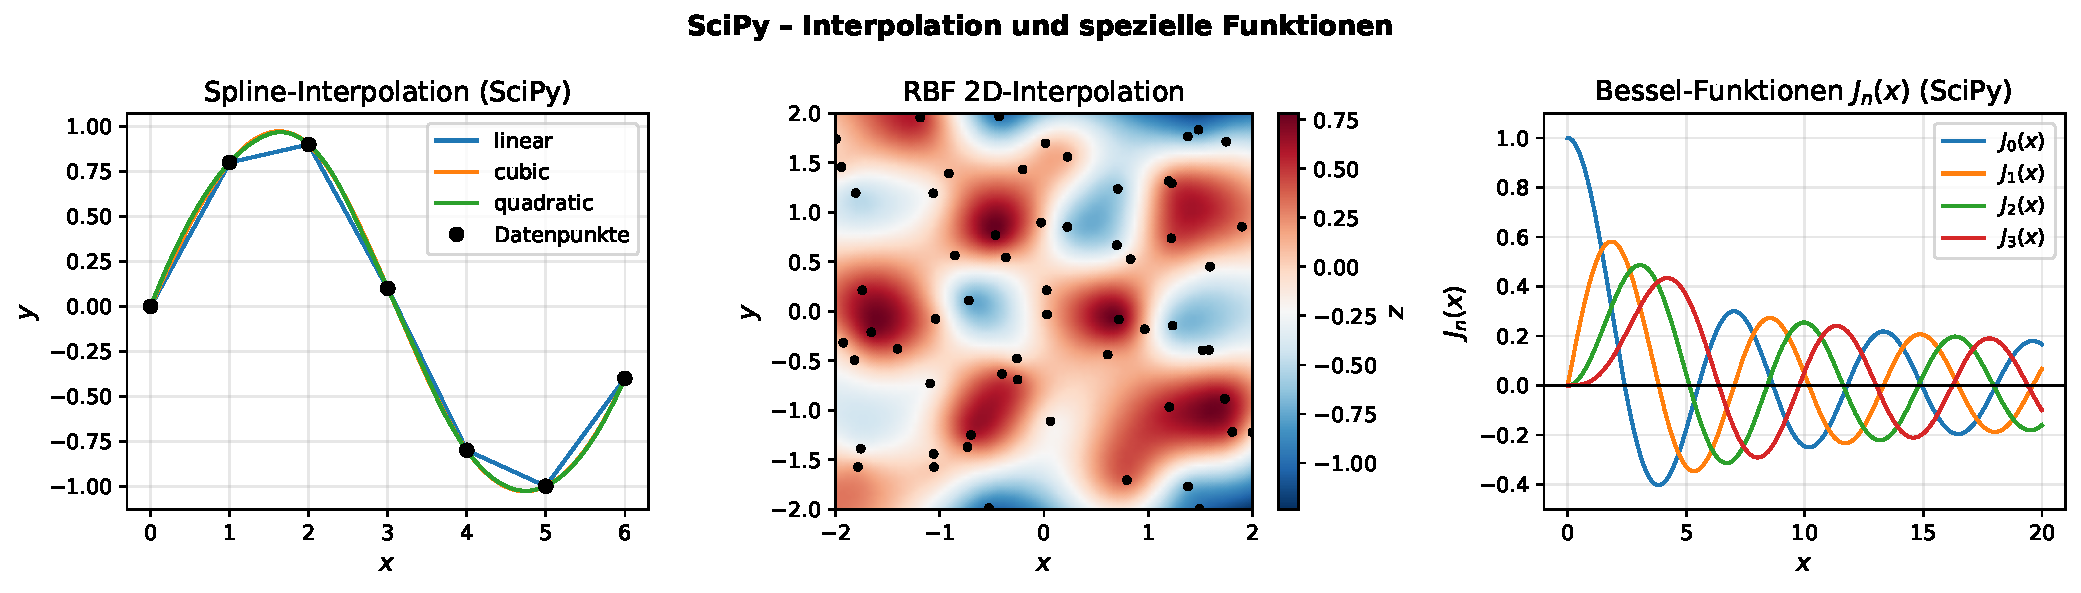
\includegraphics[width=\textwidth]{scipy_interp_special}
  \caption{SciPy Interpolation: 1D-Splines (links), 2D-RBF-Interpolation
           (Mitte), Bessel-Funktionen $J_n(x)$ (rechts).}
  \label{fig:scipy_interp_special}
\end{figure}

\subsection{Spezielle Funktionen der mathematischen Physik}
\label{subsec:scipy-special}

\texttt{scipy.special} enthält Implementierungen der wichtigsten
Funktionen der mathematischen Physik, Ingenieurswissenschaften und
Statistik \cite{abramowitz1972handbook}:

\begin{lstlisting}[caption={Spezielle Funktionen mit SciPy}]
from scipy import special
import numpy as np

x = np.linspace(0, 20, 500)

# Bessel-Funktionen (Zylindergeometrie, Wellenausbreitung)
J0 = special.jv(0, x)   # Bessel 1. Art, Ordnung 0
J1 = special.jv(1, x)
Y0 = special.yv(0, x)   # Bessel 2. Art

# Sphärische Besselfunktionen
j0_s = special.spherical_jn(0, x)

# Gamma-Funktion (Verallgemeinerung der Fakultät)
z  = np.linspace(0.1, 5, 400)
Gz = special.gamma(z)
Lz = special.loggamma(z)   # numerisch stabiler für grosse Argumente

# Legendre-Polynome (Kugelflächenfunktionen, Physik)
for n in range(5):
    Pn = special.eval_legendre(n, np.linspace(-1, 1, 200))

# Elliptische Integrale (Pendel, Gravitationslinsen)
K = special.ellipk(0.5)    # vollstaendiges elliptisches Integral K(k)
E = special.ellipe(0.5)    # vollstaendiges elliptisches Integral E(k)

# Fehler-Funktion (Wärme-/Diffusionsgleichungen)
erf_vals = special.erf(np.linspace(-3, 3, 200))

# Hypergeometrische Funktionen
hyp2f1 = special.hyp2f1(1, 2, 3, 0.5)   # Gauss'sche hypergeom. Fkt.

# Sphärische Harmonische Y_l^m
theta = np.pi/4; phi = np.pi/3
Y11 = special.sph_harm(1, 1, phi, theta)
\end{lstlisting}

\subsection{Einzigartiger Wert von SciPy}

SciPy eliminiert die Notwendigkeit, hochkomplexe numerische Algorithmen
selbst zu implementieren. Die enthaltenen Verfahren basieren auf Jahrzehnten
mathematischer Forschung (LAPACK, FITPACK, MINPACK, QUADPACK u.\,a.) und
sind in C, Fortran oder C++ implementiert – mit Python-Schnittstelle.
Ob Differentialgleichungen in der Biophysik, Signalfilterung in der
Neurologie oder Optimierungsprobleme in der Luft- und Raumfahrt:
SciPy stellt den direkten Zugang bereit.

% ==============================================================
\section{Matplotlib – Wissenschaftliche Visualisierung}
\label{sec:matplotlib}
% ==============================================================

\subsection{Architektur und Designphilosophie}
\label{subsec:mpl-arch}

Matplotlib wurde 2003 von John D. Hunter entwickelt, um MATLAB-ähnliche
Plotting-Fähigkeiten in Python bereitzustellen \cite{hunter2007matplotlib}.
Die Architektur ist in drei Schichten gegliedert:

\begin{enumerate}
  \item \textbf{Backend-Schicht}: Zuständig für das eigentliche Rendering
        (Agg, PDF, SVG, Qt5Agg, WebAgg, \ldots).
  \item \textbf{Artist-Schicht}: Alle sichtbaren Objekte (\texttt{Figure},
        \texttt{Axes}, \texttt{Line2D}, \texttt{Patch}, \ldots).
  \item \textbf{Scripting-Schicht} (\texttt{pyplot}): Zustandsbehaftete
        Komfort-API, ähnlich MATLAB.
\end{enumerate}

\begin{lstlisting}[caption={Objektbasierte Matplotlib-API (empfohlen)}]
import matplotlib.pyplot as plt
import numpy as np

fig, axes = plt.subplots(2, 3, figsize=(14, 8))
fig.suptitle('Wissenschaftliche Abbildung', fontsize=14, fontweight='bold')

x = np.linspace(0, 4*np.pi, 500)

# Linienstil, Farbe, Label
axes[0, 0].plot(x, np.sin(x), lw=2, color='tab:blue', label='$\sin(x)$')
axes[0, 0].plot(x, np.cos(x), lw=2, color='tab:orange', linestyle='--',
                label='$\cos(x)$')
axes[0, 0].set_title('Trigonometrische Funktionen')
axes[0, 0].set_xlabel('$x$'); axes[0, 0].set_ylabel('Amplitude')
axes[0, 0].legend()
axes[0, 0].grid(True, alpha=0.3)

# Feinabstimmung: Tick-Formatierung
import matplotlib.ticker as ticker
axes[0, 0].xaxis.set_major_locator(ticker.MultipleLocator(np.pi))
axes[0, 0].xaxis.set_major_formatter(
    ticker.FuncFormatter(lambda x, _: f'${x/np.pi:.0f}\\pi$')
)

plt.tight_layout()
plt.savefig('output.pdf', dpi=300, bbox_inches='tight')
\end{lstlisting}

\subsection{Grundlegende und erweiterte Diagrammtypen}
\label{subsec:mpl-types}

Abbildung~\ref{fig:matplotlib_types} zeigt eine Auswahl der wichtigsten
Diagrammtypen:

\begin{lstlisting}[caption={Vielfalt der Matplotlib-Diagrammtypen}]
import matplotlib.pyplot as plt
import numpy as np

rng = np.random.default_rng(42)

# Polarplot
fig, ax = plt.subplots(subplot_kw={'projection': 'polar'})
theta = np.linspace(0, 2*np.pi, 1000)
ax.plot(theta, np.abs(np.cos(4*theta)), label='Rosenplot')

# Histogramm mit Kerndichteschaetzung
fig, ax = plt.subplots()
data = rng.normal(0, 1, 1000)
ax.hist(data, bins=40, density=True, alpha=0.6,
        edgecolor='white', label='Histogramm')

# Boxplot mit Notch (Konfidenzintervall)
data_groups = [rng.normal(i, 1, 100) for i in range(5)]
fig, ax = plt.subplots()
bp = ax.boxplot(data_groups, notch=True, patch_artist=True,
                medianprops=dict(color='red', linewidth=2))
for patch in bp['boxes']:
    patch.set_facecolor('lightblue')

# Violin Plot
fig, ax = plt.subplots()
vp = ax.violinplot(data_groups, showmedians=True, showextrema=True)

# Stem Plot (diskrete Signale)
x_s = np.linspace(-np.pi, np.pi, 25)
fig, ax = plt.subplots()
ax.stem(x_s, np.sinc(x_s))

# Heatmap (Korrelationsmatrix)
corr = np.corrcoef(rng.normal(size=(5, 200)))
fig, ax = plt.subplots()
im = ax.imshow(corr, cmap='coolwarm', vmin=-1, vmax=1)
plt.colorbar(im, ax=ax)
\end{lstlisting}

\begin{figure}[H]
  \centering
  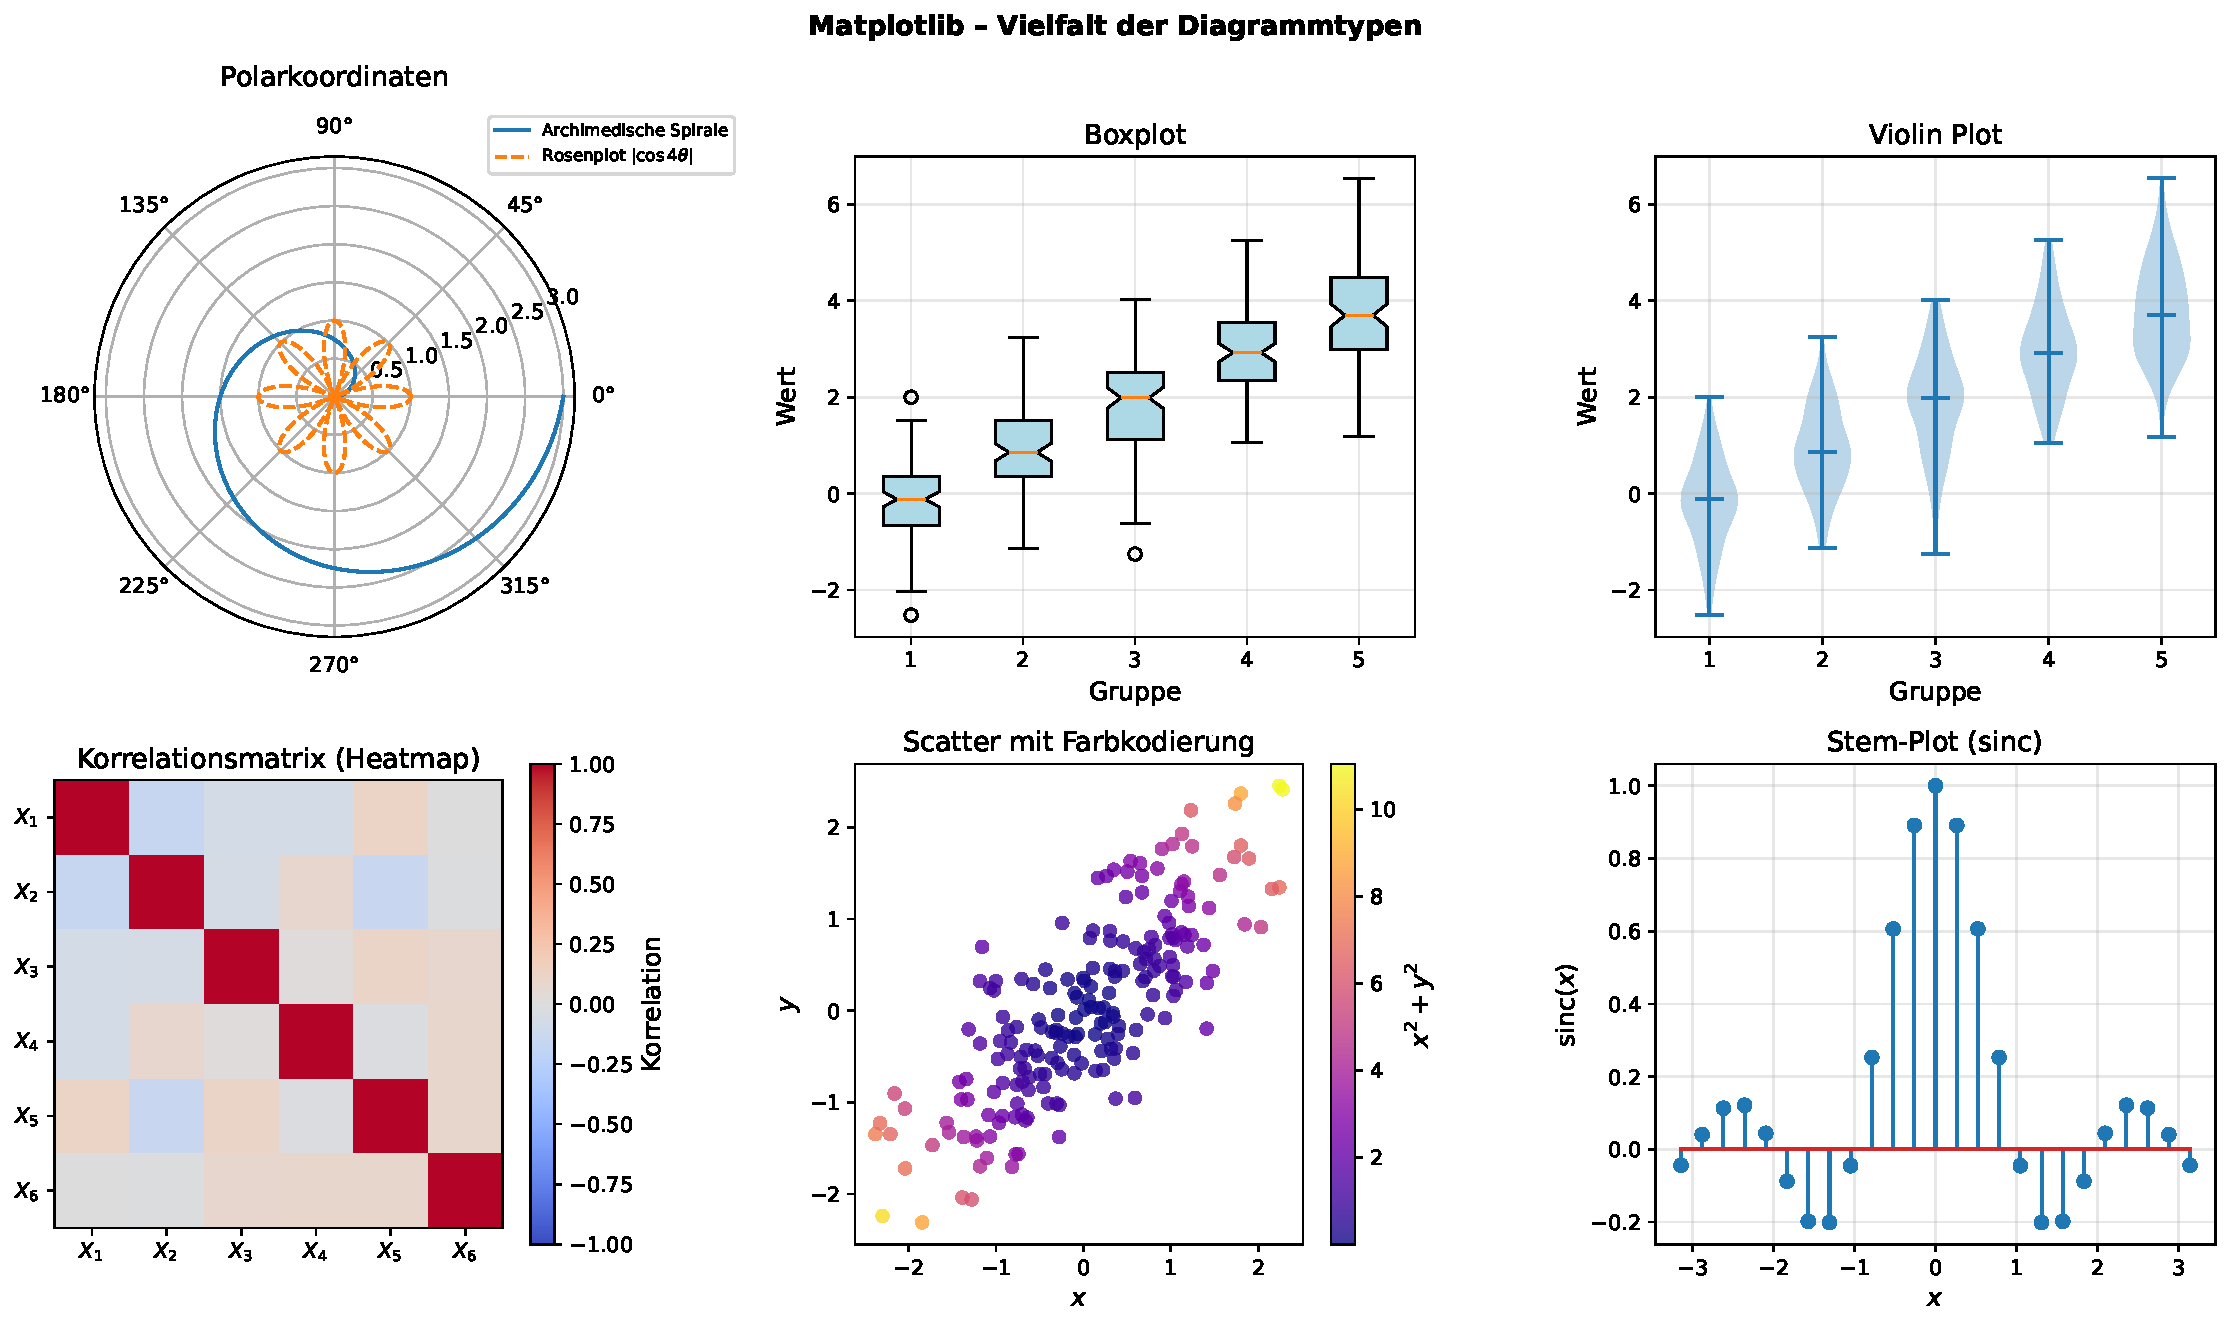
\includegraphics[width=\textwidth]{matplotlib_types}
  \caption{Matplotlib Diagrammvielfalt: Polarplot, Boxplot, Violin Plot,
           Korrelationsheatmap, Scatter mit Farbkodierung, Stem-Plot.}
  \label{fig:matplotlib_types}
\end{figure}

\subsection{3D-Visualisierung}
\label{subsec:mpl-3d}

Das Toolkit \texttt{mpl\_toolkits.mplot3d} ermöglicht reichhaltige
dreidimensionale Darstellungen:

\begin{lstlisting}[caption={3D-Visualisierung mit Matplotlib}]
from mpl_toolkits.mplot3d import Axes3D
import matplotlib.pyplot as plt
import numpy as np

fig = plt.figure(figsize=(15, 5))

# 3D-Oberfläche
ax1 = fig.add_subplot(131, projection='3d')
x = y = np.linspace(-3, 3, 80)
X, Y = np.meshgrid(x, y)
Z = np.sin(np.sqrt(X**2 + Y**2))
surf = ax1.plot_surface(X, Y, Z, cmap='viridis',
                        edgecolor='none', antialiased=True)
fig.colorbar(surf, ax=ax1, shrink=0.5)

# Drahtgitter-Plot
ax1b = fig.add_subplot(131, projection='3d')
ax1b.plot_wireframe(X, Y, Z, rstride=5, cstride=5, linewidth=0.3)

# 3D-Kontur
ax1c = fig.add_subplot(131, projection='3d')
ax1c.contourf(X, Y, Z, zdir='z', levels=20, cmap='plasma')

# Parametrische Kurve (Helix)
ax2 = fig.add_subplot(132, projection='3d')
t = np.linspace(0, 4*np.pi, 500)
ax2.plot(np.cos(t), np.sin(t), t/(4*np.pi), lw=2)

# 3D-Scatter
ax3 = fig.add_subplot(133, projection='3d')
rng = np.random.default_rng(11)
xs = rng.normal(0, 1, 200)
ys = rng.normal(0, 1, 200)
zs = xs**2 - ys**2
ax3.scatter(xs, ys, zs, c=zs, cmap='RdYlBu', s=20, alpha=0.7)
\end{lstlisting}

\begin{figure}[H]
  \centering
  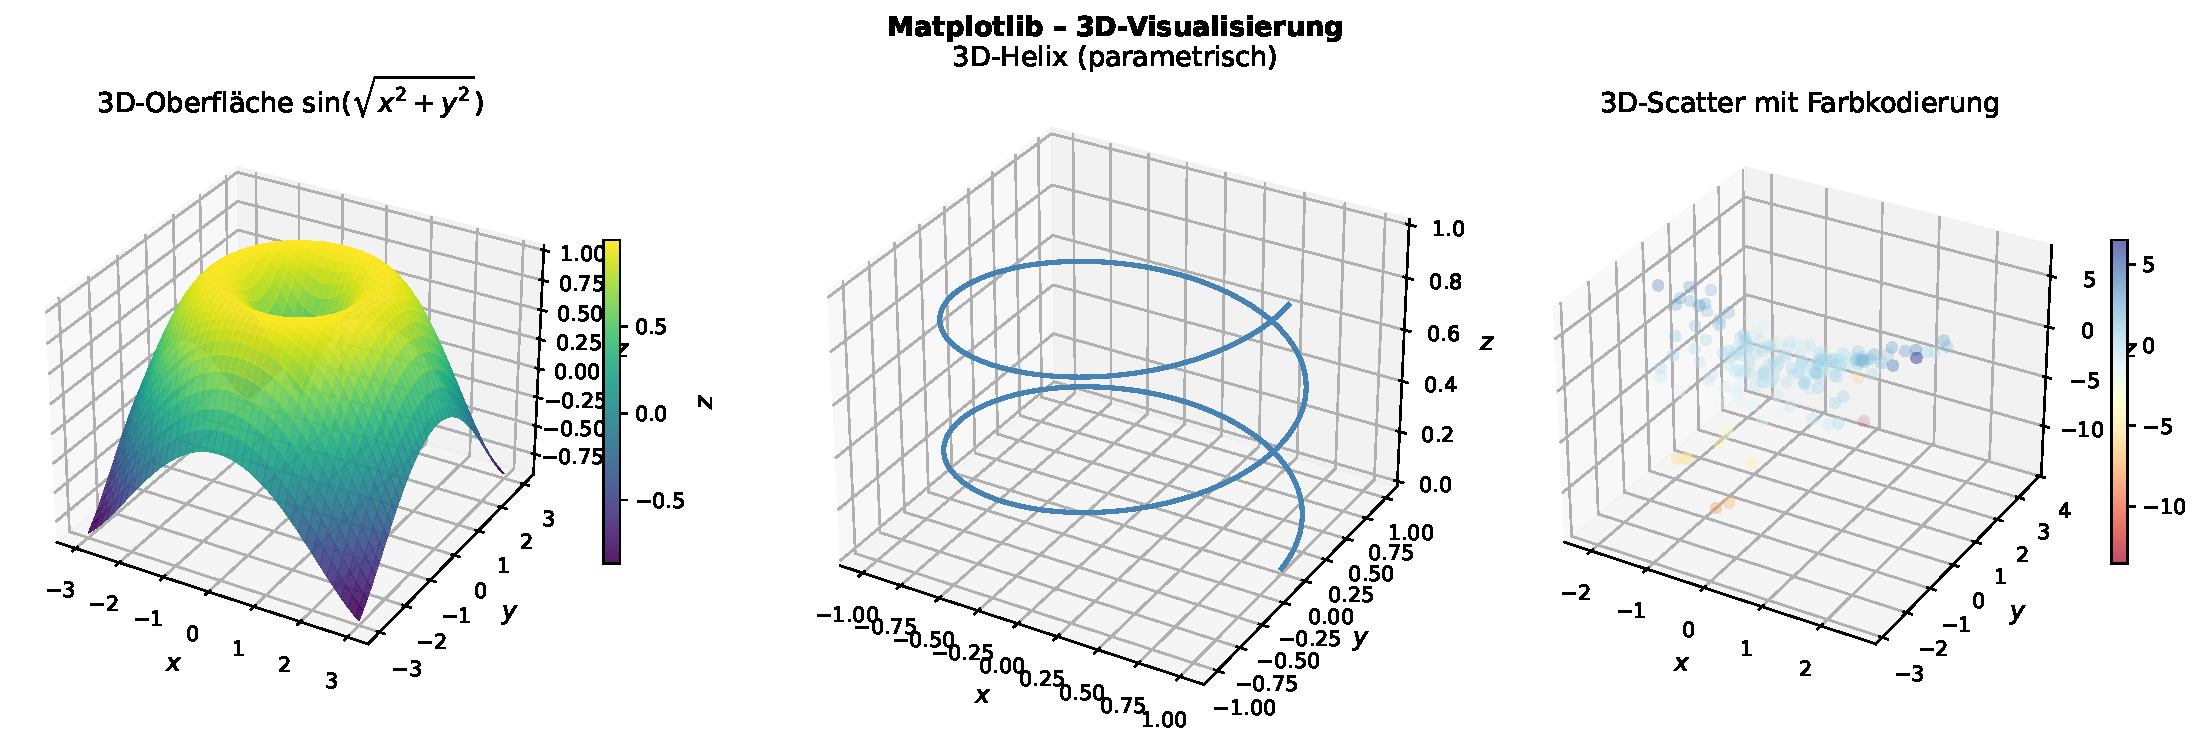
\includegraphics[width=\textwidth]{matplotlib_3d}
  \caption{Matplotlib 3D: Oberfläche $\sin(\sqrt{x^2+y^2})$ (links),
           3D-Helix als parametrische Kurve (Mitte), 3D-Scatter-
           Diagramm mit Farbkodierung (rechts).}
  \label{fig:matplotlib_3d}
\end{figure}

\subsection{Kontur-, Vektorfeld- und Stromlinienplots}
\label{subsec:mpl-contour}

\begin{lstlisting}[caption={Kontur-, Quiver- und Streamplot}]
import matplotlib.pyplot as plt
import numpy as np

x = np.linspace(-3, 3, 200)
y = np.linspace(-3, 3, 200)
X, Y = np.meshgrid(x, y)
Z = X * np.exp(-(X**2 + Y**2))

fig, axes = plt.subplots(1, 3, figsize=(14, 4))

# Gefüllter Konturplot
cf = axes[0].contourf(X, Y, Z, levels=20, cmap='RdBu_r')
axes[0].contour(X, Y, Z, levels=20, colors='k', linewidths=0.5)
plt.colorbar(cf, ax=axes[0])

# Quiver-Plot (Vektorfeld)
xq = np.linspace(-2, 2, 20); yq = np.linspace(-2, 2, 20)
XQ, YQ = np.meshgrid(xq, yq)
speed = np.sqrt((-YQ)**2 + XQ**2)
axes[1].quiver(XQ, YQ, -YQ, XQ, speed, cmap='autumn')

# Streamplot (Flusslinien)
xs = np.linspace(-3, 3, 100); ys = np.linspace(-3, 3, 100)
XS, YS = np.meshgrid(xs, ys)
speed_s = np.sqrt((-YS)**2 + XS**2)
axes[2].streamplot(xs, ys, -YS, XS, color=speed_s,
                   cmap='Blues', linewidth=1.5, density=1.5)
\end{lstlisting}

\begin{figure}[H]
  \centering
  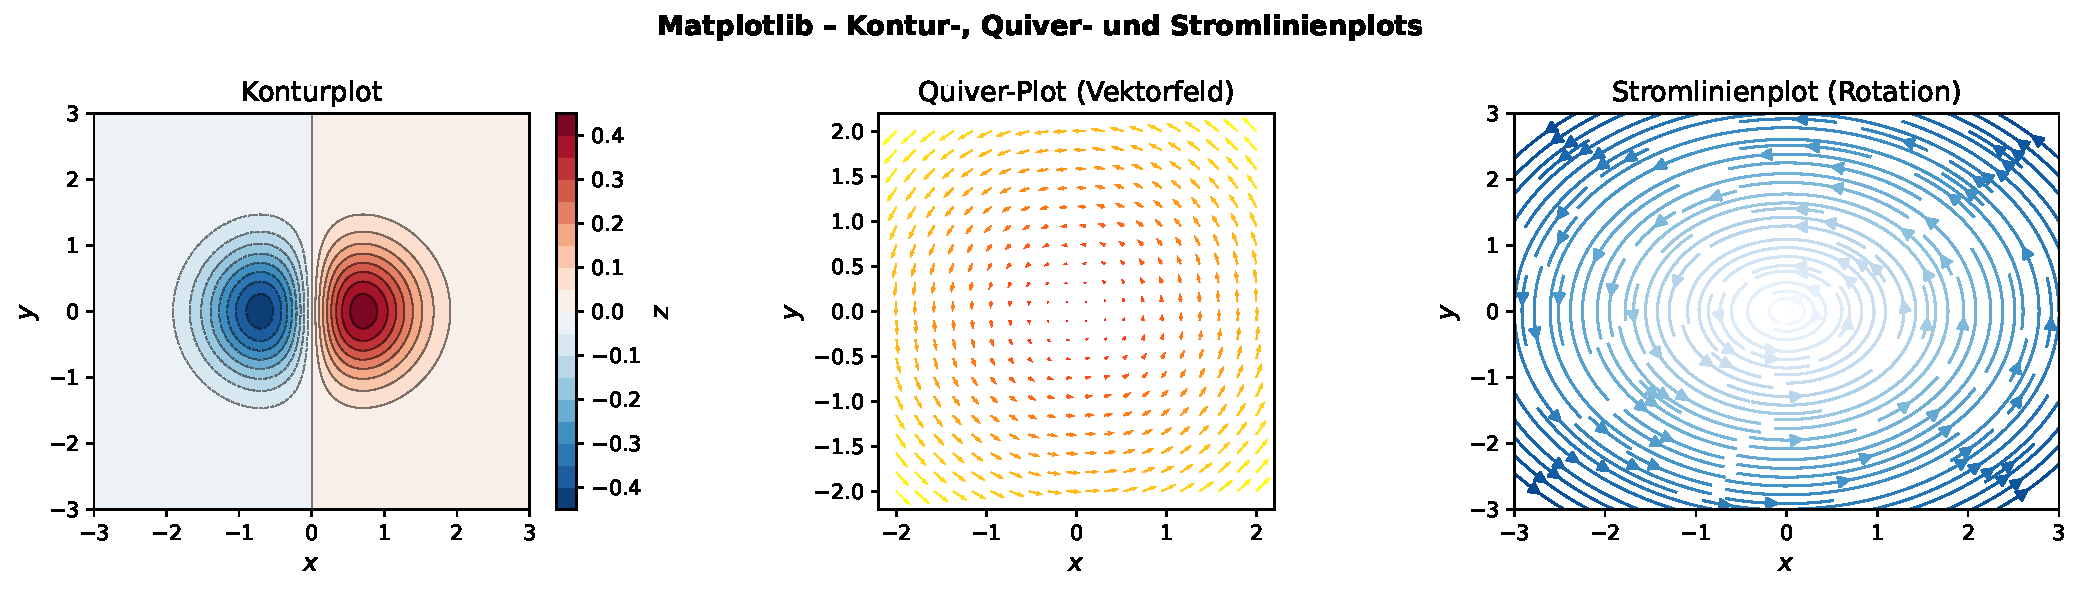
\includegraphics[width=\textwidth]{matplotlib_contour_quiver}
  \caption{Matplotlib: Konturplot (links), Quiver-Vektorfeld (Mitte),
           Stromlinienplot einer Rotationsströmung (rechts).}
  \label{fig:matplotlib_contour}
\end{figure}

\subsection{Annotationen und Unsicherheitsdarstellung}
\label{subsec:mpl-annotations}

Für wissenschaftliche Publikationen unverzichtbar ist die Darstellung von
Messunsicherheiten und die gezielte Beschriftung relevanter Merkmale:

\begin{lstlisting}[caption={Annotationen und Fehlerbaender in Matplotlib}]
import matplotlib.pyplot as plt
import numpy as np

fig, axes = plt.subplots(1, 2, figsize=(12, 4))

# Unsicherheitsband
x = np.linspace(0, 4*np.pi, 100)
y_mean = np.sin(x) * np.exp(-0.1 * x)
y_std  = 0.1 + 0.05 * np.abs(np.cos(x))

axes[0].fill_between(x, y_mean - 2*y_std, y_mean + 2*y_std,
                     alpha=0.25, label='$2\\sigma$')
axes[0].fill_between(x, y_mean - y_std,   y_mean + y_std,
                     alpha=0.4, label='$1\\sigma$')
axes[0].plot(x, y_mean, lw=2)

# Annotationen mit Pfeilen
y = np.sin(np.linspace(0, 10, 300))
max_idx = np.argmax(y)
axes[1].plot(np.linspace(0, 10, 300), y, lw=2)
axes[1].annotate('Maximum',
    xy=(np.linspace(0, 10, 300)[max_idx], y[max_idx]),
    xytext=(np.linspace(0, 10, 300)[max_idx]+1.5, 0.6),
    arrowprops=dict(arrowstyle='->', color='red', lw=1.5),
    fontsize=11, color='red'
)

# Mathematische Formeln als Text
axes[1].text(0.5, -0.8, r'$y = \sin(x)$',
             fontsize=13, transform=axes[1].transAxes,
             ha='center')
\end{lstlisting}

\begin{figure}[H]
  \centering
  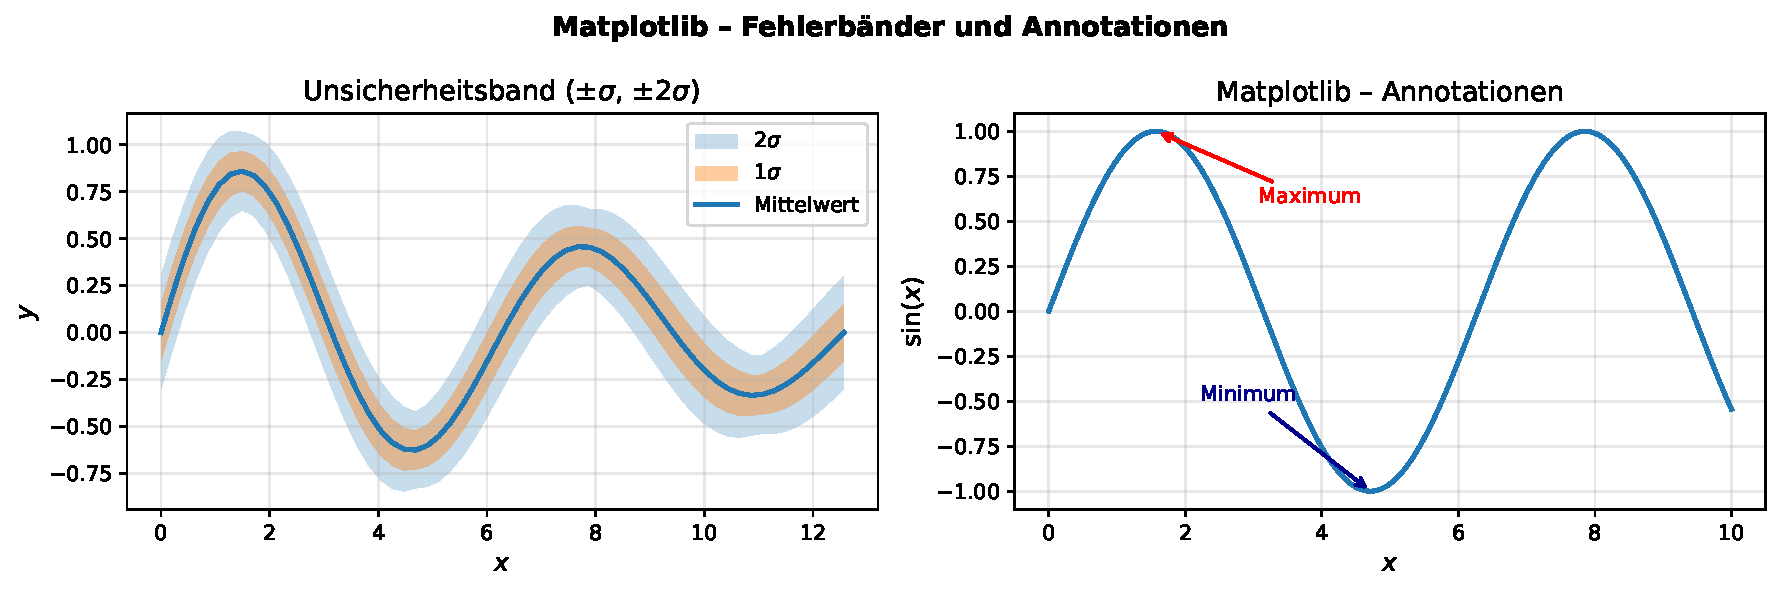
\includegraphics[width=\textwidth]{matplotlib_annotations}
  \caption{Matplotlib: $\pm\sigma$- und $\pm 2\sigma$-Unsicherheitsbänder
           (links), Annotationen mit Pfeilen (rechts).}
  \label{fig:matplotlib_annot}
\end{figure}

\subsection{Farbpaletten (Colormaps)}
\label{subsec:mpl-colormaps}

Die Wahl der Farbpalette ist entscheidend für die korrekte Wahrnehmung
wissenschaftlicher Daten. Matplotlib bietet über 80 Paletten, darunter
perzeptuell gleichförmige Karten wie \texttt{viridis}, \texttt{plasma},
\texttt{inferno} und \texttt{cividis} \cite{hunter2007matplotlib}:

\begin{lstlisting}[caption={Colormaps und barrierefreie Farbgebung}]
import matplotlib.pyplot as plt
import matplotlib.cm as cm
import numpy as np

# Alle verfügbaren Colormaps anzeigen
print(plt.colormaps())

x = y = np.linspace(-np.pi, np.pi, 100)
X, Y = np.meshgrid(x, y)
Z = np.sin(X) * np.cos(Y)

cmaps = ['viridis', 'plasma', 'inferno', 'magma',
         'cividis', 'RdBu_r', 'coolwarm', 'nipy_spectral']

fig, axes = plt.subplots(2, 4, figsize=(16, 6))
for ax, cmap in zip(axes.ravel(), cmaps):
    ax.imshow(Z, cmap=cmap, origin='lower')
    ax.set_title(cmap)
    ax.axis('off')

# Benutzerdefinierte Colormap
from matplotlib.colors import LinearSegmentedColormap
custom_cmap = LinearSegmentedColormap.from_list(
    'mein_cm', ['white', 'steelblue', 'darkblue']
)
\end{lstlisting}

\begin{figure}[H]
  \centering
  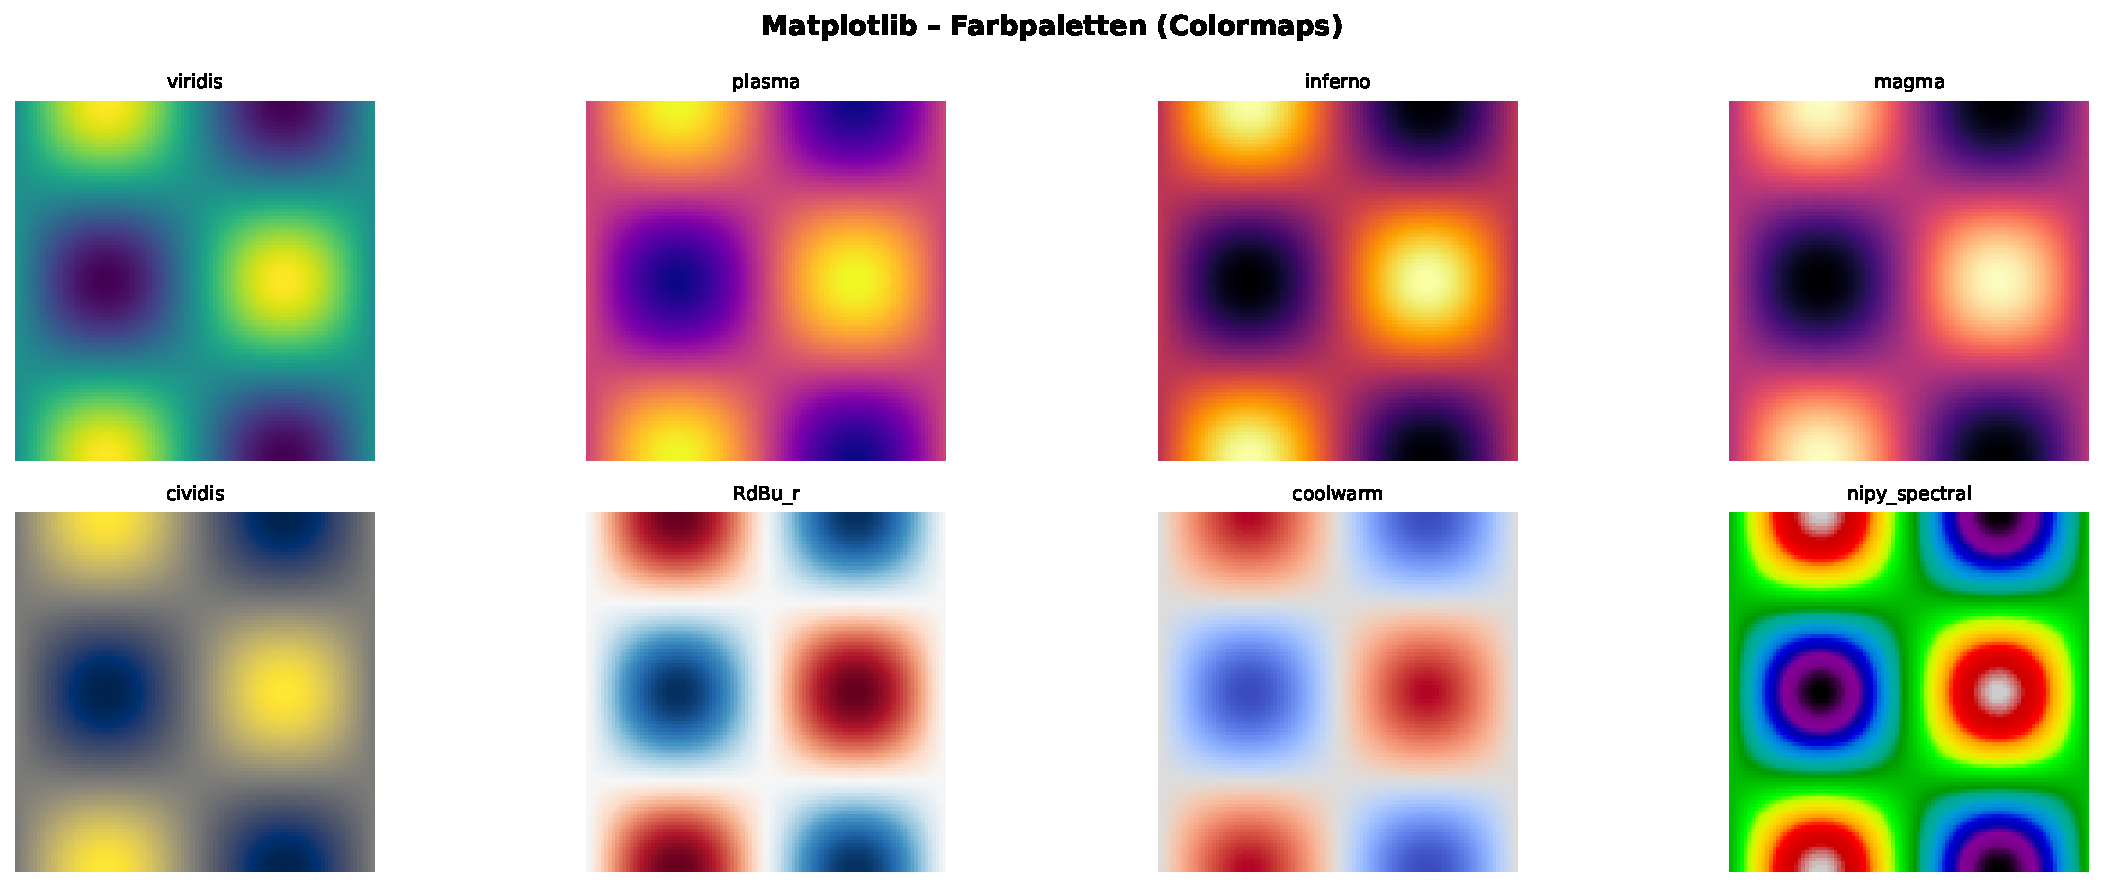
\includegraphics[width=\textwidth]{matplotlib_colormaps}
  \caption{Matplotlib Farbpaletten: Viridis, Plasma, Inferno, Magma,
           Cividis, RdBu\_r, Coolwarm und Nipy\_Spectral.}
  \label{fig:matplotlib_colormaps}
\end{figure}

\subsection{Einzigartiger Wert von Matplotlib}

Matplotlib ist das einzige Python-Visualisierungswerkzeug, das gleichzeitig
\emph{vollständige} Kontrolle über jeden Aspekt einer Grafik bietet und
dabei in allen wissenschaftlichen Backends (PDF, SVG, EPS für Journale,
PNG/TIFF für Poster) erstklassige Ausgaben erzeugt. Keine andere
Bibliothek erreicht vergleichbare typografische Qualität bei der
Ausgabe von LaTeX-gerendertem Text und mathematischen Formeln
(\texttt{usetex=True} oder \texttt{mathtext}).

% ==============================================================
\section{Zusammenspiel der Bibliotheken: Anwendungsbeispiele}
\label{sec:applications}
% ==============================================================

\subsection{Nichtlineare Dynamik: Das Lorenz-System}
\label{subsec:lorenz}

Das Lorenz-System \cite{lorenz1963deterministic} ist das Paradigma des
deterministischen Chaos:
\begin{align}
  \dot{x} &= \sigma(y - x),\\
  \dot{y} &= x(\rho - z) - y,\\
  \dot{z} &= xy - \beta z,
\end{align}
mit den klassischen Parametern $\sigma=10$, $\rho=28$, $\beta=8/3$.

\begin{lstlisting}[caption={Lorenz-Attraktor mit NumPy, SciPy und Matplotlib}]
import numpy as np
from scipy import integrate
import matplotlib.pyplot as plt

def lorenz(t, state, sigma=10, rho=28, beta=8/3):
    x, y, z = state
    return [sigma*(y-x), x*(rho-z)-y, x*y-beta*z]

# Numerische Lösung (SciPy solve_ivp)
sol = integrate.solve_ivp(
    lorenz, (0, 50), [1, 1, 1],
    t_eval=np.linspace(0, 50, 20000),
    method='RK45', max_step=0.01
)

# Visualisierung (Matplotlib)
fig = plt.figure(figsize=(12, 5))
ax1 = fig.add_subplot(121, projection='3d')
ax1.plot(sol.y[0], sol.y[1], sol.y[2], lw=0.3, alpha=0.7)
ax1.set_title('Lorenz-Attraktor (3D)')

# Leistungsspektrum (NumPy FFT)
ax2 = fig.add_subplot(122)
freqs = np.fft.rfftfreq(len(sol.t), d=50/20000)
power = np.abs(np.fft.rfft(sol.y[0]))**2
ax2.semilogy(freqs[1:1000], power[1:1000])
ax2.set_title('Leistungsspektrum (Lorenz $x$)')
\end{lstlisting}

\begin{figure}[H]
  \centering
  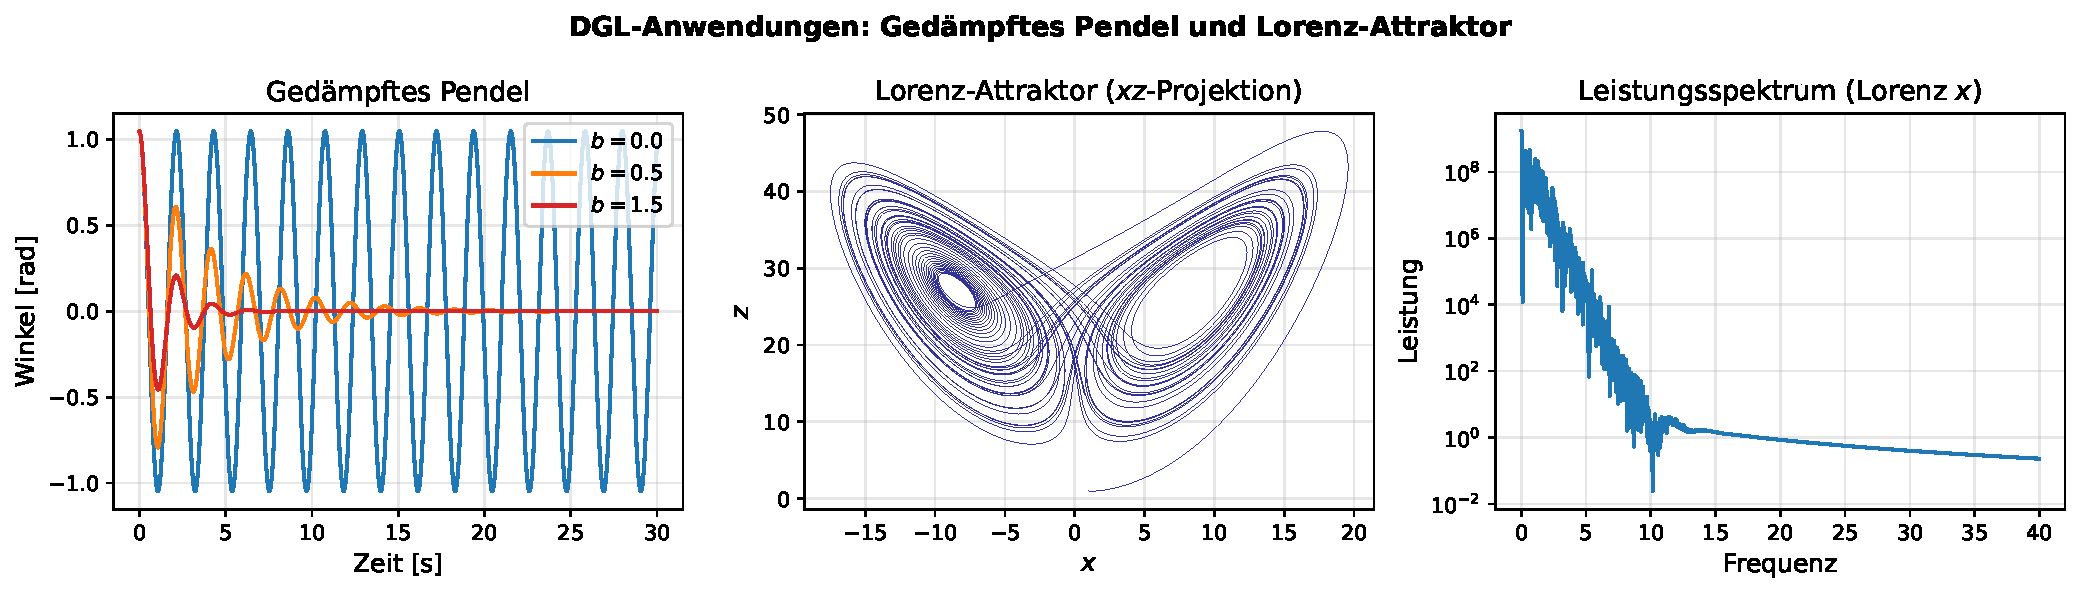
\includegraphics[width=\textwidth]{pendulum_lorenz}
  \caption{DGL-Anwendungen: Gedämpftes Pendel (links), Lorenz-Attraktor
           (Mitte), Leistungsspektrum der $x$-Komponente (rechts).}
  \label{fig:pendulum_lorenz}
\end{figure}

\subsection{Wärmeleitungsgleichung: Spektralmethode}
\label{subsec:heat}

Die eindimensionale Wärmeleitungsgleichung
\begin{equation}
  \frac{\partial u}{\partial t} = \alpha \frac{\partial^2 u}{\partial x^2}
\end{equation}
kann mit NumPys FFT exakt und effizient (spektrale Methode) gelöst werden:

\begin{lstlisting}[caption={PDE-Loesung via FFT (NumPy)}]
import numpy as np

N = 256;  L = 2*np.pi;  alpha = 0.01
x = np.linspace(0, L, N, endpoint=False)
u = np.exp(-4*(x - np.pi)**2)   # Gauss-Anfangsbedingung

k = np.fft.rfftfreq(N) * N * (2*np.pi/L)  # Wellenzahlen
dt = 0.01;  n_steps = 500
u_hat = np.fft.rfft(u)

snapshots = [u.copy()]
for i in range(n_steps):
    u_hat *= np.exp(-alpha * k**2 * dt)   # exakte spektrale Propagation
    if (i+1) % 100 == 0:
        snapshots.append(np.fft.irfft(u_hat))

# Bildverarbeitung: Gauss-Glättung als Wärmediffusion
from scipy.ndimage import gaussian_filter
image = np.zeros((100, 100))
image[30:70, 30:70] = 1.0
blurred = gaussian_filter(image, sigma=5)
\end{lstlisting}

\begin{figure}[H]
  \centering
  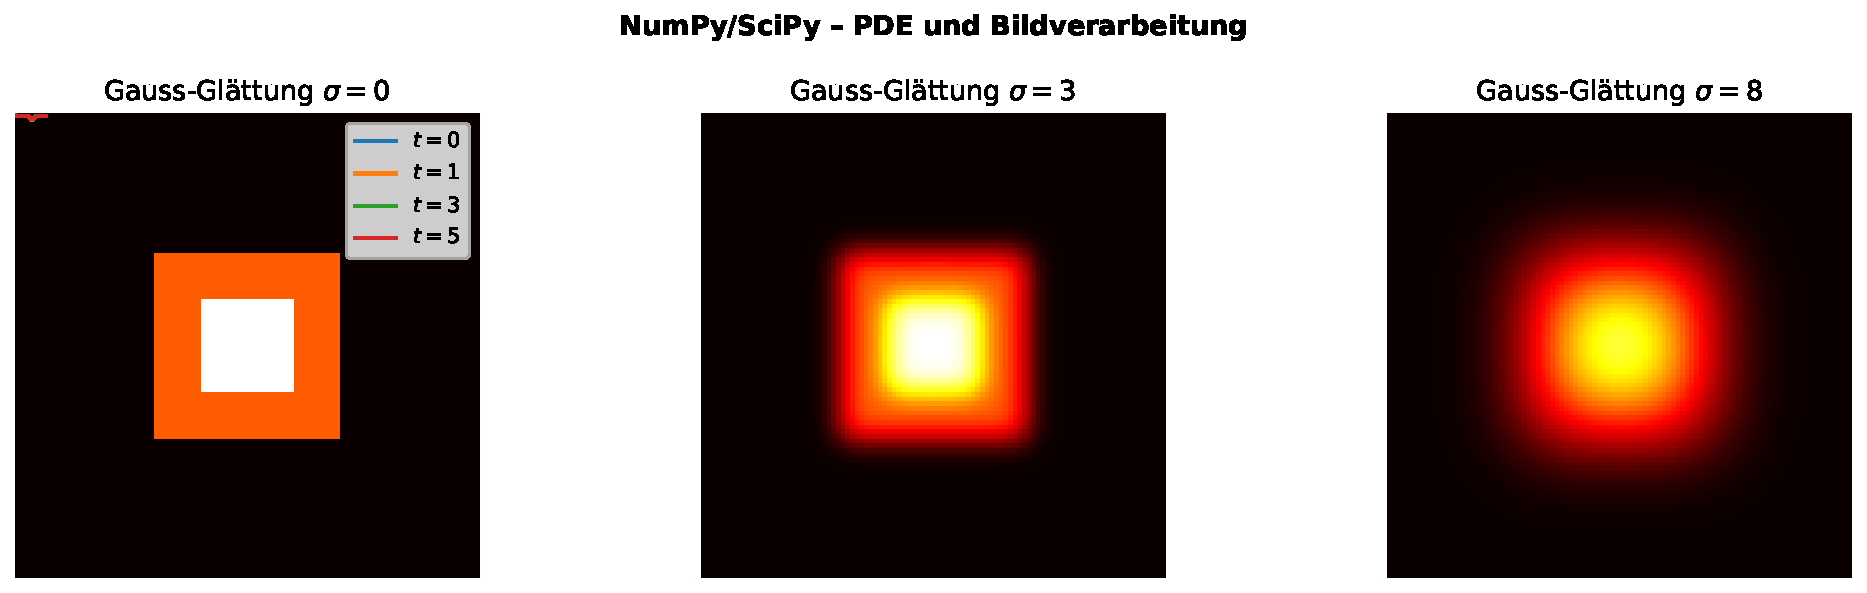
\includegraphics[width=\textwidth]{pde_image}
  \caption{PDE und Bildverarbeitung: Gauss-Glättung mit $\sigma=0, 3, 8$
           als Analogie zur Wärmeleitung.}
  \label{fig:pde_image}
\end{figure}

\subsection{Zusammenfassende Bewertung}
\label{subsec:zusammenfassung}

\begin{table}[H]
  \centering
  \begin{tabular}{llll}
    \toprule
    \textbf{Aufgabe} & \textbf{NumPy} & \textbf{SciPy} & \textbf{Matplotlib} \\
    \midrule
    Array-Operationen      & \checkmark\checkmark\checkmark & \checkmark & -- \\
    FFT/Spektralanalyse    & \checkmark\checkmark & \checkmark\checkmark\checkmark & -- \\
    Lineare Algebra        & \checkmark\checkmark & \checkmark\checkmark\checkmark & -- \\
    Optimierung            & -- & \checkmark\checkmark\checkmark & -- \\
    DGL-Lösung             & -- & \checkmark\checkmark\checkmark & -- \\
    Statistik              & \checkmark & \checkmark\checkmark\checkmark & -- \\
    Interpolation          & \checkmark & \checkmark\checkmark\checkmark & -- \\
    2D-Plots               & -- & -- & \checkmark\checkmark\checkmark \\
    3D-Plots               & -- & -- & \checkmark\checkmark \\
    Publikationsqualität   & -- & -- & \checkmark\checkmark\checkmark \\
    \bottomrule
  \end{tabular}
  \caption{Stärken (\checkmark\checkmark\checkmark = hauptverantwortlich,
           \checkmark = unterstützend, -- = nicht primär) der drei Bibliotheken
           in den wichtigsten wissenschaftlichen Aufgabenbereichen.}
  \label{tab:comparison}
\end{table}

% ==============================================================
\section{Leistungsmessung und Skalierbarkeit}
\label{sec:performance}
% ==============================================================

Ein wesentlicher Vorteil dieser Bibliotheken liegt in ihrer Effizienz.
Tabelle~\ref{tab:perf} zeigt exemplarische Geschwindigkeitsvergleiche
zwischen reinem Python und NumPy/SciPy:

\begin{table}[H]
  \centering
  \begin{tabular}{lrrl}
    \toprule
    \textbf{Operation} & \textbf{Reines Python} & \textbf{NumPy/SciPy} & \textbf{Speedup} \\
    \midrule
    Summe ($10^7$ Elemente) & ca. 1\,000 ms & ca. 8 ms & ${\approx}125\times$ \\
    Matmul ($1000\times1000$) & ca. 300\,s & ca. 0.06 s & ${\approx}5\,000\times$ \\
    FFT ($2^{20}$ Punkte) & N/A (manuell) & ca. 120 ms & $\gg$ \\
    Sortierung ($10^6$) & ca. 800 ms & ca. 60 ms & ${\approx}13\times$ \\
    ODE-Lösung (RK45) & ca. 60\,s & ca. 0.1 s & ${\approx}600\times$ \\
    \bottomrule
  \end{tabular}
  \caption{Exemplarische Laufzeitvergleiche auf einem modernen Laptop
           (Intel i7, 16\,GB RAM). Die Werte sind Richtwerte und können
           je nach Hardware variieren \cite{vanderplas2016python}.}
  \label{tab:perf}
\end{table}

% ==============================================================
\section{Schlussfolgerung}
\label{sec:conclusion}
% ==============================================================

Die vorliegende Arbeit hat gezeigt, dass \textbf{NumPy}, \textbf{SciPy}
und \textbf{Matplotlib} zusammen eine vollständige, hochleistungsfähige
und ausdrucksstarke Infrastruktur für das wissenschaftliche Rechnen mit
Python bilden. Ihre Bedeutung lässt sich in drei Dimensionen fassen:

\begin{enumerate}
  \item \textbf{Ausdrucksstärke}: Die Bibliotheken ermöglichen die
  Formulierung komplexer mathematischer Konzepte (Eigenwertzerlegungen,
  DGL-Systeme, Faltungsfilter, spezielle Funktionen) in wenigen, les-
  baren Python-Zeilen.
  
  \item \textbf{Effizienz}: Durch C/Fortran-Backends und Algorithmen
  aus jahrzehntelanger numerischer Forschung sind die Implementierungen
  oft mit spezialisierter Forschungssoftware vergleichbar oder überlegen.
  
  \item \textbf{Ökosystem}: Als Bausteine von Pandas, scikit-learn,
  TensorFlow, Astropy, BioPython u.\,v.\,a. sind diese drei Bibliotheken
  die gemeinsame Sprache der wissenschaftlichen Python-Gemeinschaft.
\end{enumerate}

Die Anwendungsbeispiele – vom Lorenz-Attraktor über die spektrale PDE-Lösung
bis hin zu statistischen Tests und Signalfiltern – belegen eindrücklich, dass
das wissenschaftliche Arbeiten ohne das Trio NumPy/SciPy/Matplotlib in der
heutigen Form kaum vorstellbar wäre. Zukünftige Entwicklungen wie
\texttt{CuPy} (GPU-NumPy), \texttt{JAX} (differenzierbares NumPy) und
\texttt{SciPy.fft} (FFTW-Backend) werden auf demselben konzeptionellen
Fundament aufbauen und zeigen, dass die hier dargelegten Prinzipien
zeitlos und zukunftssicher sind \cite{bradbury2018jax}.

% ==============================================================
\subsection{Ausblick: Entwicklungstendenzen und Zukunftsperspektiven}
\label{subsec:ausblick}
% ==============================================================

Die vorstehende Analyse hat gezeigt, dass \textbf{NumPy}, \textbf{SciPy}
und \textbf{Matplotlib} in ihrer heutigen Form bereits einen außerordentlichen
Reifegrad besitzen. Gleichwohl ist das wissenschaftliche Python-Ökosystem
kein statisches Gebilde, sondern ein dynamisches, sich kontinuierlich
weiterentwickelndes System, das auf Herausforderungen der Praxis reagiert.
Im Folgenden werden die bedeutendsten Entwicklungstendenzen und
Zukunftsperspektiven ausführlich dargelegt, die das wissenschaftliche
Rechnen mit Python in den kommenden Jahren grundlegend prägen werden.

% ------------------------------------------------------------------
\subsubsection{GPU-Beschleunigung und heterogenes Rechnen}
\label{subsubsec:gpu}
% ------------------------------------------------------------------

Die rasante Verbreitung von Grafikprozessoren (GPUs) in Forschung und
Industrie hat eine neue Klasse von NumPy-kompatiblen Bibliotheken
hervorgebracht, die nahezu identische Schnittstellen bieten, die
Berechnungen aber auf GPU-Hardware ausführen.

\textbf{CuPy} \cite{cupy2017} stellt eine direkte Drop-in-Ersetzung für
NumPy auf NVIDIA-CUDA-Hardware bereit. Für Matrizen der Größe
$10\,000 \times 10\,000$ erreicht CuPy bei Matrixmultiplikationen
Speedups von $100\times$ gegenüber NumPy auf der CPU. Die Migration
eines bestehenden NumPy-Codes erfordert in vielen Fällen lediglich den
Austausch des Import-Statements:

\begin{lstlisting}[caption={CuPy als Drop-in-Ersatz fuer NumPy}]
# Vorher:  import numpy as np
import cupy as np   # identische API, GPU-Ausfuehrung

A = np.random.normal(size=(5000, 5000))
B = np.linalg.svd(A)   # laeuft auf GPU
\end{lstlisting}

\textbf{ROCm/HIP} (AMD) und \textbf{Metal} (Apple Silicon) erweitern
den Horizont über NVIDIA-Hardware hinaus. Bibliotheken wie
\texttt{PyOpenCL} und \texttt{ArrayFire} erlauben hardwareagnostisches
GPU-Computing. Mittelfristig ist zu erwarten, dass SciPy und NumPy selbst
optionale GPU-Backends über das standardisierte Array-API-Protokoll
(siehe Abschnitt~\ref{subsubsec:array-api}) unterstützen werden.

Neben der GPU-Beschleunigung gewinnt auch das sogenannte \emph{heterogene
Rechnen} an Bedeutung: Rechenaufgaben werden dabei dynamisch auf die
optimale Hardwareeinheit verteilt – CPU-Kerne für seriell-sequentielle
Teilprobleme, GPUs für massiv-parallele Matrix- und Tensoroperationen,
und spezialisierte Beschleuniger wie FPGAs oder TPUs für besonders
häufig wiederkehrende Routinen. Die Fähigkeit von NumPy, als gemeinsame
konzeptuelle Sprache für all diese Plattformen zu dienen, macht das Array
zu einem universellen Abstrakt ionsinstrument.

% ------------------------------------------------------------------
\subsubsection{JAX: Differenzierbares Programmieren und JIT-Kompilierung}
\label{subsubsec:jax}
% ------------------------------------------------------------------

\textbf{JAX} \cite{bradbury2018jax} von Google DeepMind ist die bislang
weitreichendste Erweiterung des NumPy-Paradigmas. Es kombiniert vier
transformative Fähigkeiten in einer einzigen Bibliothek:

\begin{enumerate}
  \item \textbf{Automatische Differentiation (\texttt{jax.grad})}: Jede
    in NumPy-Stil geschriebene Funktion kann automatisch abgeleitet
    werden – sowohl Vorwärts- als auch Rückwärtsmodus. Dies ermöglicht
    die Implementierung von Gradientenabstiegsverfahren, adjungierten
    Methoden für PDE-Optimierung und Sensitivitätsanalysen, ohne dass
    analytische Ableitungen manuell hergeleitet werden müssen.

  \item \textbf{JIT-Kompilierung (\texttt{jax.jit})}: Funktionen werden
    bei erstem Aufruf durch die XLA-Compiler-Pipeline übersetzt und
    erreichen dadurch Ausführungsgeschwindigkeiten nahe am theoretischen
    Hardware-Limit.

  \item \textbf{Vektorisierung (\texttt{jax.vmap})}: Eine für ein einzelnes
    Element geschriebene Funktion wird automatisch auf ganze Batches von
    Eingaben vektorisiert, ohne explizite Schleifen.

  \item \textbf{Parallelisierung (\texttt{jax.pmap})}: Code wird
    automatisch auf mehrere GPU- oder TPU-Einheiten verteilt.
\end{enumerate}

\begin{lstlisting}[caption={JAX: Automatische Differentiation und JIT}]
import jax
import jax.numpy as jnp

def potential(q):
    """Harmonisches Potential: V(q) = 0.5 * q^2"""
    return 0.5 * jnp.dot(q, q)

# Gradient  dV/dq analytisch korrekt
grad_V = jax.grad(potential)

# Hessematrix  d^2V/dq^2
hess_V = jax.jacfwd(jax.grad(potential))

# JIT-Kompilierung
@jax.jit
def simulation_step(q, p, dt=0.01):
    force = -grad_V(q)
    p_new = p + dt * force
    q_new = q + dt * p_new
    return q_new, p_new

# Vektorisierung ueber 1000 Trajektorien gleichzeitig
batched_step = jax.vmap(simulation_step)
\end{lstlisting}

Die Konsequenz dieser Fähigkeiten ist fundamental: Physikalische Modelle,
die zuvor nur als \emph{Forward}-Simulationen ausgeführt werden konnten,
werden durch JAX zu differenzierbaren Programmen, deren Parameter durch
gradientenbasierte Optimierungsverfahren kalibriert werden können. Dies
öffnet die Tür zu einem neuen Paradigma des \emph{Scientific Machine
Learning}, das numerische Simulation und maschinelles Lernen organisch
verbindet.

% ------------------------------------------------------------------
\subsubsection{Physik-informierte neuronale Netze (PINNs)}
\label{subsubsec:pinn}
% ------------------------------------------------------------------

Eine der bedeutsamsten Entwicklungen an der Schnittstelle von maschinellem
Lernen und numerischer Mathematik ist das Konzept der
\emph{Physics-Informed Neural Networks} (PINNs). Dabei werden neuronale
Netze nicht nur durch Daten, sondern auch durch die Residuen bekannter
partieller Differentialgleichungen (PDEs) trainiert. Das Netz approximiert
die Lösung der PDE direkt als Funktion der Raumzeit-Koordinaten.

NumPy und SciPy spielen bei PINNs eine doppelte Rolle: Erstens als
Werkzeuge zur Datengenerierung, Gittererstellung und Referenzlösung;
zweitens als Backend für Bibliotheken wie \texttt{DeepXDE} oder
\texttt{NeuralPDE.jl}, die auf NumPy-kompatiblen Array-Operationen aufbauen.

Die Navier-Stokes-Gleichungen, Schrödinger-Gleichungen, Diffusionsgleichungen
und Maxwell-Gleichungen werden derzeit aktiv als PINN-Benchmarks untersucht.
Zukünftig ist zu erwarten, dass SciPy-Löser als Kollokationspunktgeneratoren
und Referenzlöser für den Trainingsprozess von PINNs dienen werden, während
Matplotlib zur Visualisierung der gelernten Lösungsfelder unverzichtbar bleibt.

% ------------------------------------------------------------------
\subsubsection{Numba und Cython: Just-in-Time-Kompilierung für Python}
\label{subsubsec:numba}
% ------------------------------------------------------------------

Für Algorithmen, die sich nicht vollständig vektorisieren lassen und
explizite Schleifen erfordern, bieten \textbf{Numba} und \textbf{Cython}
komplementäre Ansätze zur Beschleunigung:

\begin{lstlisting}[caption={Numba: JIT-Kompilierung von Python-Schleifen}]
from numba import njit, prange
import numpy as np

@njit(parallel=True)
def stencil_diffusion(u, alpha, dt, dx):
    """Finite-Differenzen-Diskretisierung der Waermeleitung."""
    n = len(u)
    u_new = np.empty_like(u)
    for i in prange(1, n - 1):    # parallel ueber alle inneren Punkte
        u_new[i] = u[i] + alpha * dt / dx**2 * (u[i+1] - 2*u[i] + u[i-1])
    u_new[0]  = u[0]              # Randbedingung links
    u_new[-1] = u[-1]             # Randbedingung rechts
    return u_new
\end{lstlisting}

Numba kompiliert die mit \texttt{@njit} dekorierten Funktionen bei erstem
Aufruf durch LLVM zu nativem Maschinencode. Schleifen, die in reinem Python
um den Faktor $1\,000$ langsamer wären als die entsprechende C-Implementierung,
erreichen nach Numba-Kompilierung nahezu identische Laufzeiten. Dies ist
besonders relevant für iterative PDE-Löser, Graphalgorithmen und
Monte-Carlo-Simulationen, bei denen Broadcasting kein vollständiges
Vektorisierungsäquivalent ermöglicht.

Mittelfristig werden Numba und NumPy noch stärker integriert werden:
Das \textbf{NumPy Enhancement Proposal 47 (NEP~47)} schlägt eine
standardisierte \texttt{\_\_array\_namespace\_\_}-Schnittstelle vor, die
Numba-JIT-kompilierte Funktionen transparent über beliebige Array-Backends
hinweg auführbar macht.

% ------------------------------------------------------------------
\subsubsection{Paralleles und verteiltes Rechnen: Dask und Ray}
\label{subsubsec:dask}
% ------------------------------------------------------------------

Sobald Datensätze den verfügbaren Arbeitsspeicher überschreiten oder
Berechnungen auf Cluster-Infrastrukturen verteilt werden sollen, greifen
Wissenschaftler zunehmend auf \textbf{Dask} zurück. Dask stellt verteilte
Äquivalente zu NumPy-Arrays und Pandas-DataFrames bereit, wobei die
Berechnungen als azyklische Abhängigkeitsgraphen (DAGs) modelliert und
lazy ausgewertet werden:

\begin{lstlisting}[caption={Dask: Out-of-Core-NumPy fuer gro\ss{}e Datensaetze}]
import dask.array as da
import numpy as np

# 100 GB grosses Array -- wird nie vollstaendig in den RAM geladen
x = da.random.normal(size=(100_000, 100_000), chunks=(1_000, 1_000))

# Berechnung wird lazy aufgebaut
result = (x * x).mean(axis=0)

# Erst hier: parallele Ausfuehrung auf allen CPU-Kernen
result_computed = result.compute()
\end{lstlisting}

\textbf{Ray} wiederum ermöglicht die feingranulare Verteilung beliebiger
Python-Funktionen auf Cluster-Knoten und bietet mit \texttt{Ray Tune}
eine skalierbare Hyperparameter-Optimierungsplattform, die intern auf
SciPy-Optimierungsroutinen zurückgreift.

\textbf{Xarray} erweitert NumPy-Arrays um benannte Dimensionen und
Koordinaten (ähnlich wie NetCDF-Dateien) und ist zur Standardbibliothek
der Klima- und Ozeanografiewissenschaften geworden. In Verbindung mit
Dask ermöglicht Xarray die Verarbeitung von petabytegroßen Klimasimulationsdaten.

Zu erwarten ist, dass diese Out-of-Core- und Distributed-Computing-
Lösungen zunehmend direkt in SciPy und NumPy integriert werden, sodass
der Übergang zwischen lokalem und verteiltem Rechnen für den Endanwender
transparent und reibungslos gestaltet wird.

% ------------------------------------------------------------------
\subsubsection{Das Array-API-Protokoll und Bibliotheks-Interoperabilität}
\label{subsubsec:array-api}
% ------------------------------------------------------------------

Eines der ambitioniertesten aktuellen Vorhaben im Scientific-Python-
Ökosystem ist die Standardisierung einer einheitlichen \emph{Array-API},
die von der Python-Datenwissenschafts-Community unter dem Dach der
\emph{Python Array API Standard}-Initiative (ehemals NEP~47) vorangetrieben
wird.

Das Ziel ist es, eine minimale, aber ausreichend reichhaltige Menge von
Array-Operationen zu definieren, die von allen bedeutenden Array-
Bibliotheken – NumPy, CuPy, JAX, PyTorch, TensorFlow, Dask, cuDF –
implementiert werden. Bibliotheken wie SciPy, die auf dieser Schnittstelle
aufbauen, könnten dann transparent auf allen unterstützten Backends
ausgeführt werden, ohne den Quellcode zu ändern:

\begin{lstlisting}[caption={Array-API-kompatible SciPy-Funktion (Zukunftsvision)}]
# Hypothetisches Beispiel fuer Array-API-transparentes SciPy
import scipy.linalg as la

# Dasselbe SVD laeuft auf NumPy-Array (CPU)
import numpy as np
A_cpu = np.random.normal(size=(1000, 1000))
U, s, Vt = la.svd(A_cpu)     # Ausfuehrung auf CPU

# ... und auf CuPy-Array (GPU) -- kein Codechange
import cupy as cp
A_gpu = cp.random.normal(size=(1000, 1000))
U_gpu, s_gpu, Vt_gpu = la.svd(A_gpu)  # Ausfuehrung auf GPU
\end{lstlisting}

SciPy hat mit Version~1.11 begonnen, Array-API-Kompatibilität in
ausgewählten Submodulen (\texttt{scipy.special}, \texttt{scipy.fft})
zu implementieren, und plant die schrittweise Erweiterung auf alle
Kernbereiche. Dies hat das Potenzial, SciPy zu einem vollständig
hardwareagnostischen wissenschaftlichen Algorithmen-Stack zu machen.

% ------------------------------------------------------------------
\subsubsection{Symbolisch-numerische Hybridmethoden}
\label{subsubsec:sympy}
% ------------------------------------------------------------------

Die Integration symbolischer Mathematik (durch \textbf{SymPy}) mit
numerischer Berechnung (durch NumPy und SciPy) hat sich zu einem eigenen
Forschungsfeld entwickelt. \textbf{Lambdify} und \textbf{codegen} in SymPy
überführen symbolisch hergeleitete Ausdrücke in numerisch auswertbaren
Python-, NumPy- oder Fortran-Code:

\begin{lstlisting}[caption={SymPy + NumPy: Symbolisch-numerische Pipeline}]
from sympy import symbols, sin, diff, lambdify, Matrix
import numpy as np

x, t = symbols('x t')
omega = symbols('omega', positive=True)

# Symbolische Herleitung der Dispersionsrelation
u = sin(x - omega * t)
phase_velocity = omega / (x.diff(x))   # Symbolisch

# Jacobi-Matrix eines nichtlinearen Systems
F = Matrix([x**2 + t*x - 1, x*t - t**2])
J = F.jacobian([x, t])
print("Jacobi-Matrix:", J)

# Numerisch auswertbar via lambdify (NumPy-Backend)
jacobian_num = lambdify([x, t], J, modules='numpy')
J_values = jacobian_num(np.linspace(0, 1, 100), 0.5)
\end{lstlisting}

Zukünftige Entwicklungen werden die Symbiose von SymPy und SciPy
vertiefen: Automatisch generierte Jacobimatrizen für SciPy-Optimierer,
symbolisch hergeleitete Vorkonditionierer für lineare Gleichungssysteme
und analytisch bekannte Integrationskerne für numerische Quadratur sind
nur einige der vielversprechenden Anknüpfungspunkte.

% ------------------------------------------------------------------
\subsubsection{Interaktive und webbasierte Visualisierung}
\label{subsubsec:interactive-viz}
% ------------------------------------------------------------------

Matplotlib hat seinen Ursprung in der Erzeugung statischer,
druckbereiter Abbildungen. Die zunehmende Verlagerung wissenschaftlicher
Arbeit in browserbasierte Umgebungen (Jupyter Lab, VS~Code, Google Colab)
und interaktive Dashboards hat eine neue Generation von Visualisierungs-
werkzeugen hervorgebracht, die auf den Konzepten von Matplotlib aufbauen
oder mit ihr interagieren:

\begin{description}
  \item[\textbf{Plotly}] bietet deklarative, interaktive Grafiken mit
    Zoom, Hover-Tooltips und verknüpften Ansichten. Die Plotly-Express-API
    folgt eng der Matplotlib-Semantik und ermöglicht die Migration
    bestehender Matplotlib-Workflows.

  \item[\textbf{Bokeh}] ist auf datengetriebene Webanwendungen und
    Streaming-Daten optimiert und ermöglicht die Einbettung wissenschaft-
    licher Visualisierungen in HTML-Seiten ohne serverseitige Infrastruktur.

  \item[\textbf{HoloViews / HvPlot}] abstrahiert über verschiedene
    Visualisierungs-Backends (Matplotlib, Bokeh, Plotly) und erlaubt
    die deklarative Beschreibung von Datensichten, deren konkrete
    Darstellung vom gewählten Backend abhängt.

  \item[\textbf{ipywidgets + Matplotlib}] ermöglichen vollständig
    interaktive Parameterstudien in Jupyter-Notebooks: Schieberegler,
    Dropdown-Menüs und Textfelder steuern direkt die Parameter von
    NumPy/SciPy-Berechnungen und aktualisieren die Matplotlib-Darstellung
    in Echtzeit.

  \item[\textbf{WebAssembly / Pyodide}] transportiert den gesamten
    Scientific-Python-Stack – einschließlich NumPy, SciPy und Matplotlib
    – direkt in den Webbrowser. Bildungsinstitutionen berichten bereits
    von vollständig serverlos betriebenen interaktiven Lern-Umgebungen.
\end{description}

Matplotlib selbst antwortet auf diese Entwicklungen durch erweiterte
Backend-Unterstützung (\texttt{ipympl}/\texttt{widget}-Backend für
Jupyter) und ein zunehmend feingranulares Artist-Modell, das programmatische
Animationen und interaktive Elemente erleichtert. Zu erwarten ist, dass
Matplotlib als Rendering-Grundlage für höherschichtige interaktive
Frameworks bestehen bleibt, während die direkte Nutzung für statische
Publikationsgrafiken weiterhin unübertroffen ist.

% ------------------------------------------------------------------
\subsubsection{Wissenschaftliches maschinelles Lernen und datengetriebene
Modellentdeckung}
\label{subsubsec:sciml}
% ------------------------------------------------------------------

Die Verbindung zwischen klassischen numerischen Methoden und modernem
maschinellem Lernen manifestiert sich in einem rasch wachsenden Feld,
das unter den Bezeichnungen \emph{Scientific Machine Learning} (SciML)
oder \emph{AI for Science} bekannt ist. NumPy, SciPy und Matplotlib
nehmen dabei eine Doppelrolle ein: als Werkzeuge zur Datenerzeugung und
-vorverarbeitung einerseits, und als Referenzimplementierungen, gegen
die lernbasierte Ansätze validiert werden, andererseits.

Konkrete Entwicklungsfelder umfassen:

\begin{itemize}
  \item \textbf{Sparse Identification of Nonlinear Dynamics (SINDy)}:
    Datengetriebene Herleitung von Differentialgleichungen aus Zeitreihen.
    NumPy-basierte Bibliotheken wie \texttt{PySINDy} rekonstruieren aus
    Messdaten automatisch die dominanten Terme eines DGL-Systems –
    etwa die Lotka-Volterra-Gleichungen aus simulierten Populationsdaten,
    ohne a-priori-Kenntnis des Modells.

  \item \textbf{Operatorlernen (DeepONet, Fourier Neural Operator)}:
    Neuronale Netze, die anstelle von Funktionswerten ganze Lösungsoperatoren
    von PDEs lernen. SciPy-Löser erzeugen die Trainingsdaten; die gelernten
    Operatoren können anschließend Vorhersagen $10^4$-mal schneller als
    traditionelle Löser liefern.

  \item \textbf{Bayesianische Optimierung mit SciPy als Unterbau}:
    Bibliotheken wie \texttt{scikit-optimize} und \texttt{GPyOpt}
    verwenden \texttt{scipy.optimize} für interne Akquisitionsfunktions-
    Optimierungen und \texttt{scipy.stats} für die Beschreibung von
    Prioris.

  \item \textbf{Normalizing Flows und differenzierbare Simulationen}:
    NumPy-Daten treiben das Training von Wahrscheinlichkeitsdichte-
    Abschätzungsmodellen in der Astro- und Teilchenphysik.
\end{itemize}

% ------------------------------------------------------------------
\subsubsection{Reproduzierbare Wissenschaft und FAIR-Datenprinzipien}
\label{subsubsec:fair}
% ------------------------------------------------------------------

Mit der wachsenden Veröffentlichungspflicht für Forschungsdaten und
-code gewinnen Fragen der Reproduzierbarkeit wissenschaftlicher Ergebnisse
an institutioneller Bedeutung \cite{donoho2010invitation, peng2011reproducible}.
NumPy, SciPy und Matplotlib reagieren auf diese Herausforderung durch
mehrere strukturelle Eigenschaften:

\begin{description}
  \item[\textbf{Semantische Versionierung und Deprecation-Policies}]:
    Alle drei Bibliotheken folgen strikten Versionierungsrichtlinien, die
    mehrjährige Rückwärtskompatibilität gewährleisten. Wissenschaftliche
    Paper, deren Berechnungen auf NumPy~1.x basieren, können durch
    \texttt{pip install numpy==1.26} reproduziert werden.

  \item[\textbf{Zitierbarkeit}]: Mit den DOI-verlinkten Nature-Publikationen
    \cite{harris2020array, virtanen2020scipy, hunter2007matplotlib} sind
    alle drei Bibliotheken vollständig zitierfähig, ein wichtiger Meilenstein
    für ihre Anerkennung als Forschungsinfrastruktur.

  \item[\textbf{Jupyter und nbformat}]: Das standardisierte Notebook-Format
    ermöglicht die vollständige Einbettung von NumPy/SciPy/Matplotlib-
    basierten Analysen in reproduzierbare, ausführbare Dokumente. Mit
    \texttt{nbconvert} und \texttt{papermill} können diese automatisiert
    ausgeführt werden.

  \item[\textbf{FAIR-kompatible Datenformate}]: \texttt{scipy.io} liest und
    schreibt HDF5- und NetCDF-Dateien, die den FAIR-Datenprinzipien
    (Findable, Accessible, Interoperable, Reusable) genügen.
    Ergänzende Bibliotheken wie \texttt{zarr} und \texttt{h5py} bauen
    direkt auf NumPy-Arrays auf.
\end{description}

Zukünftige Entwicklungen werden die Integration mit dem verbreiteten
Daten-Repository-Dienst \textbf{Zenodo} und dem Open-Science-Framework
\textbf{OSF} stärken, sodass NumPy/SciPy-Analysen direkt aus dem Code
heraus mit persistenten Identifikatoren archiviert werden können.

% ------------------------------------------------------------------
\subsubsection{Hochleistungsrechnen und Exascale-Computing}
\label{subsubsec:hpc}
% ------------------------------------------------------------------

Die Ära des \emph{Exascale-Computing} – mit Systemen, die mehr als
$10^{18}$ Gleitkommaoperationen pro Sekunde ausführen – stellt das
wissenschaftliche Python-Ökosystem vor neuartige Herausforderungen.
Auf Maschinen mit Hunderttausenden von CPU-Kernen und Tausenden von
GPU-Knoten sind herkömmliche NumPy-Arrays inadequat. Dennoch bilden sie
die konzeptuelle Grundlage für eine neue Generation von HPC-Abstraktionen:

\begin{itemize}
  \item \textbf{mpi4py + NumPy}: Die Pythonbindung des Message Passing
    Interface (MPI) überträgt NumPy-Array-Segmente direkt zwischen
    Rechenknoten, ohne Datenkopien. NumPy-basierter Code läuft dadurch
    auf Supercomputern mit wenigen hundert Zeilen Boilerplate.

  \item \textbf{PETSc / SLEPc Python-Interfaces}: Ãœber \texttt{petsc4py}
    sind die weltführenden Bibliotheken für skalierbare lineare Algebra
    und Eigenwertprobleme aus Python nutzbar – mit NumPy-Arrays als
    Daten-Ãœbergabeschnittstelle.

  \item \textbf{FEniCSx und Firedrake}: Finite-Elemente-Frameworks für
    großskalige PDE-Simulationen integrieren NumPy/SciPy als Postprocessing-
    und Visualisierungs-Backend über \texttt{pyvista} und Matplotlib.

  \item \textbf{PyFR und OpenFOAM Python-Bindings}: Strömungsmechanik-
    Codes der industriellen und akademischen Spitzenforschung bieten
    zunehmend Python-Schnittstellen, die NumPy-Arrays als primäres
    Datenformat verwenden.
\end{itemize}

Langfristig wird erwartet, dass SciPy dedizierte Parallelversionen
seiner Kernalgorithmen einführt – verteilte FFTs (basierend auf
\texttt{pfft} oder \texttt{mpiFFT4py}), parallele Gleichungslöser
und skalierbare Optimierungsroutinen.

% ------------------------------------------------------------------
\subsubsection{Quantencomputing und Quanten-Simulation}
\label{subsubsec:quantum}
% ------------------------------------------------------------------

Das Aufkommen von Quantencomputern mit 100--1\,000 physischen Qubits
eröffnet völlig neue Möglichkeiten für die wissenschaftliche Berechnung.
NumPy und SciPy spielen in diesem Kontext eine doppelte Rolle:

Einerseits sind sie die primären Werkzeuge für die \emph{klassische Simulation
von Quantensystemen}. Bibliotheken wie \textbf{QuTiP} (Quantum Toolbox in
Python) verwenden dichte NumPy-Matrizen und SciPy-Eigenwertlöser, um
Hamiltonoperatoren, Dichtematrizen und Lindbladgleichungen für offene
Quantensysteme zu berechnen:

\begin{lstlisting}[caption={QuTiP: Quantendynamik mit NumPy/SciPy}]
import qutip as qt
import numpy as np

# Zwei-Niveau-System (Qubit)
H = qt.sigmax()                   # Hamiltonoperator: sigma_x
psi0 = qt.basis(2, 0)             # Anfangszustand |0>

tlist = np.linspace(0, 10, 200)   # Zeitvektor (NumPy)
# Schroedinger-Gleichung loesen (intern: SciPy solve_ivp)
result = qt.mesolve(H, psi0, tlist, [], [qt.sigmax(), qt.sigmaz()])

# Erwartungswerte visualisieren (Matplotlib)
import matplotlib.pyplot as plt
plt.plot(tlist, result.expect[0], label=r'$\langle\sigma_x\rangle$')
plt.plot(tlist, result.expect[1], label=r'$\langle\sigma_z\rangle$')
\end{lstlisting}

Andererseits bieten \textbf{Qiskit} (IBM), \textbf{Cirq} (Google) und
\textbf{PennyLane} Python-Schnittstellen für echte Quanten-Hardware, die
intern NumPy für die Darstellung von Quantenzustandsvektoren und
Messstatistiken nutzen. Mit der Konsolidierung der Quantenhardware wird
NumPy als gemeinsames Datenformat die Brücke zwischen klassischer und
Quantenberechnung bilden.

% ------------------------------------------------------------------
\subsubsection{Nachhaltigkeit und Community-Governance des Ökosystems}
\label{subsubsec:governance}
% ------------------------------------------------------------------

Eine oft unterschätzte Dimension der Zukunftsperspektiven betrifft nicht
die technologische, sondern die soziale und institutionelle Nachhaltigkeit
des Scientific-Python-Ökosystems. Die vergangenen Jahre haben gezeigt,
dass hochwertige Open-Source-Infrastruktur für die Wissenschaft dauerhafter
Finanzierung und stabiler Governance bedarf:

\begin{description}
  \item[\textbf{NumFOCUS}]: Die gemeinnützige Organisation finanziert und
    koordiniert die Entwicklung von NumPy, SciPy, Matplotlib und über
    40 weiteren wissenschaftlichen Python-Projekten durch Förderanträge,
    Konferenzen (SciPy~Conference, PyData) und Unternehmenssponsoring.

  \item[\textbf{SPEC-Prozess (Scientific Python Ecosystem Coordination)}]:
    Die \emph{Scientific Python Ecosystem Coordination}-Dokumente
    standardisieren Versionierungsrichtlinien, Python-Mindestversionen
    und Interoperabilitätsnormen für alle Mitgliedsprojekte, um den
    enormen Koordinationsaufwand eines verteilten Ökosystems zu reduzieren.

  \item[\textbf{Förderinstitutionen}]: Der Chan Zuckerberg Initiative
    \emph{Essential Open Source for Science}-Fonds und das Alfred~P.~Sloan
    Foundation \emph{Scientific Software}-Programm finanzieren Vollzeit-
    Entwicklerstellen für NumPy, SciPy und Matplotlib.

  \item[\textbf{Diversität und Inklusion}]: Gezielte Programme wie
    \emph{GSoC} (Google Summer of Code) und \emph{Outreachy} erweitern
    den Entwicklerpool und stellen sicher, dass das Ökosystem die
    Anforderungen einer global diverse wissenschaftlichen Gemeinschaft
    widerspiegelt.
\end{description}

Die langfristige Perspektive ist optimistisch: Das dreifache Fundament aus
technischer Exzellenz, institutioneller Verankerung und einer wachsenden,
engagierten Community garantiert, dass NumPy, SciPy und Matplotlib nicht
nur kurzfristige Werkzeuge, sondern dauerhafter Bestandteil der
wissenschaftlichen Infrastruktur bleiben werden.

% ------------------------------------------------------------------
\subsubsection{Synthese: Eine unverzichtbare und zukunftssichere Plattform}
\label{subsubsec:synthese}
% ------------------------------------------------------------------

Die vorstehenden Ausblicke auf GPU-Beschleunigung, differenzierbares
Programmieren, maschinelles Lernen, Quantencomputing und Exascale-HPC
verdeutlichen eine übergeordnete Erkenntnis: Alle diese Entwicklungslinien
bauen auf denselben konzeptuellen Grundlagen auf, die NumPy, SciPy und
Matplotlib vor mehr als zwei Jahrzehnten etabliert haben – das
N-dimensionale Array als universelle Datenstruktur, hochoptimierte
Algorithmen aus der numerischen Mathematik und publikationsreife
Visualisierung als kommunikatives Endprodukt wissenschaftlicher Arbeit.

Jede neue Bibliothek – ob JAX, CuPy, Dask oder PyTorch – definiert ihre
Schnittstellen in exakter Analogie zu NumPy, jeder neue Algorithmen-Stack
orientiert sich an SciPy, und jede visualisierungsorientierte Anwendung
erbt Designentscheidungen von Matplotlib. Dies ist keine Zufälligkeit,
sondern Ausdruck tief verwurzelter Qualität: Diese drei Bibliotheken haben
durch jahrzehntelangen Einsatz in allen Gebieten der Wissenschaft bewiesen,
dass ihre Abstraktionen die richtige Granularität besitzen, um sowohl
universell als auch performant zu sein.

Das Scientific-Python-Ökosystem steht nicht am Ende einer Entwicklung,
sondern am Beginn einer neuen Phase, in der die bewährten Prinzipien von
NumPy, SciPy und Matplotlib auf heterogene Hardware, differenzierbares
Rechnen, künstliche Intelligenz und planetare Datenskalen ausgedehnt werden.
Wer heute NumPy, SciPy und Matplotlib beherrscht, hält den
Generalschlüssel zu diesem gesamten zukünftigen Ökosystem in Händen.

% ==============================================================
%  AUSFÃœHRLICHE QUELLENANGABE
% ==============================================================

\addcontentsline{toc}{section}{Literaturverzeichnis}
\begin{thebibliography}{99}

% ----------------------------------------------------------------
% NumPy – Primäre Quellen
% ----------------------------------------------------------------

\bibitem{harris2020array}
C.~R. Harris, K.~J. Millman, S.~J. van der Walt \textit{et al.}
Array programming with {NumPy}.
\textit{Nature}, 585(7825):357--362, 2020.
\url{https://doi.org/10.1038/s41586-020-2649-2}

\bibitem{oliphant2006guide}
T.~E. Oliphant.
\textit{A Guide to {NumPy}}.
Trelgol Publishing, 2006.
\url{https://numpy.org/doc/stable/}

\bibitem{oliphant2007numpy}
T.~E. Oliphant.
Python for Scientific Computing.
\textit{Computing in Science \& Engineering}, 9(3):10--20, 2007.
\url{https://doi.org/10.1109/MCSE.2007.58}

\bibitem{vanderplas2016python}
J. VanderPlas.
\textit{Python Data Science Handbook}.
O'Reilly Media, 2016.
\url{https://jakevdp.github.io/PythonDataScienceHandbook/}

\bibitem{mckinney2017python}
W. McKinney.
\textit{Python for Data Analysis}, 2.~Auflage.
O'Reilly Media, 2017.

% ----------------------------------------------------------------
% SciPy – Primäre Quellen
% ----------------------------------------------------------------

\bibitem{virtanen2020scipy}
P. Virtanen, R. Gommers, T.~E. Oliphant \textit{et al.}
{SciPy} 1.0: Fundamental Algorithms for Scientific Computing in Python.
\textit{Nature Methods}, 17:261--272, 2020.
\url{https://doi.org/10.1038/s41592-019-0686-2}

\bibitem{jones2001scipy}
E. Jones, T.~E. Oliphant, P. Peterson \textit{et al.}
{SciPy}: Open Source Scientific Tools for Python, 2001.
\url{https://www.scipy.org/}

% ----------------------------------------------------------------
% Matplotlib – Primäre Quellen
% ----------------------------------------------------------------

\bibitem{hunter2007matplotlib}
J.~D. Hunter.
Matplotlib: A {2D} Graphics Environment.
\textit{Computing in Science \& Engineering}, 9(3):90--95, 2007.
\url{https://doi.org/10.1109/MCSE.2007.55}

\bibitem{dale2015data}
K. Dale, S. Murray und V. Tolochko.
\textit{Data Visualization with Python and JavaScript}.
O'Reilly Media, 2015.

\bibitem{devert2014matplotlib}
A. Devert.
\textit{matplotlib Plotting Cookbook}.
Packt Publishing, 2014.

% ----------------------------------------------------------------
% Bücher zum Scientific Python Stack
% ----------------------------------------------------------------

\bibitem{numerical2020}
R. Johansson.
\textit{Numerical Python: Scientific Computing and Data Science
Applications with NumPy, SciPy and Matplotlib}, 2.~Auflage.
Apress, 2019.
\url{https://doi.org/10.1007/978-1-4842-4246-4}

\bibitem{langtangen2016primer}
H.~P. Langtangen.
\textit{A Primer on Scientific Programming with Python}, 5.~Auflage.
Springer, 2016.
\url{https://doi.org/10.1007/978-3-662-49887-3}

\bibitem{scopatz2015effective}
A. Scopatz und K.~D. Huff.
\textit{Effective Computation in Physics}.
O'Reilly Media, 2015.

% ----------------------------------------------------------------
% Numerische Mathematik
% ----------------------------------------------------------------

\bibitem{press2007numerical}
W.~H. Press, S.~A. Teukolsky, W.~T. Vetterling und B.~P. Flannery.
\textit{Numerical Recipes: The Art of Scientific Computing}, 3.~Auflage.
Cambridge University Press, 2007.

\bibitem{golub2013matrix}
G.~H. Golub und C.~F. van Loan.
\textit{Matrix Computations}, 4.~Auflage.
Johns Hopkins University Press, 2013.

\bibitem{trefethen-spectral}
L.~N. Trefethen.
\textit{Spectral Methods in MATLAB}.
SIAM, 2000.
\url{https://doi.org/10.1137/1.9780898719598}

\bibitem{burden2015numerical}
R.~L. Burden, J.~D. Faires und A.~M. Burden.
\textit{Numerical Analysis}, 10.~Auflage.
Cengage Learning, 2015.

\bibitem{atkinson1989introduction}
K.~E. Atkinson.
\textit{An Introduction to Numerical Analysis}, 2.~Auflage.
John Wiley \& Sons, 1989.

% ----------------------------------------------------------------
% Signalverarbeitung
% ----------------------------------------------------------------

\bibitem{oppenheim2010discrete}
A.~V. Oppenheim und R.~W. Schafer.
\textit{Discrete-Time Signal Processing}, 3.~Auflage.
Prentice Hall, 2010.

\bibitem{lyons2011understanding}
R.~G. Lyons.
\textit{Understanding Digital Signal Processing}, 3.~Auflage.
Prentice Hall, 2011.

\bibitem{cooley1965algorithm}
J.~W. Cooley und J.~W. Tukey.
An algorithm for the machine calculation of complex {Fourier} series.
\textit{Mathematics of Computation}, 19(90):297--301, 1965.
\url{https://doi.org/10.1090/S0025-5718-1965-0178586-1}

% ----------------------------------------------------------------
% Statistik
% ----------------------------------------------------------------

\bibitem{hastie2009elements}
T. Hastie, R. Tibshirani und J. Friedman.
\textit{The Elements of Statistical Learning}, 2.~Auflage.
Springer, 2009.
\url{https://doi.org/10.1007/978-0-387-84858-7}

\bibitem{grinstead2012introduction}
C.~M. Grinstead und J.~L. Snell.
\textit{Introduction to Probability}, 2.~Auflage.
American Mathematical Society, 2012.
\url{https://math.dartmouth.edu/~prob/prob/prob.pdf}

\bibitem{wasserstein1968bayes}
M.~H. DeGroot und M.~J. Schervish.
\textit{Probability and Statistics}, 4.~Auflage.
Pearson, 2012.

% ----------------------------------------------------------------
% Differentialgleichungen und Dynamische Systeme
% ----------------------------------------------------------------

\bibitem{lotka1925elements}
A.~J. Lotka.
\textit{Elements of Physical Biology}.
Williams and Wilkins, 1925.

\bibitem{volterra1926variazioni}
V. Volterra.
Variazioni e fluttuazioni del numero d'individui in specie animali conviventi.
\textit{Mem.~Accad.~Lincei Roma}, 2:31--113, 1926.

\bibitem{lorenz1963deterministic}
E.~N. Lorenz.
Deterministic Nonperiodic Flow.
\textit{Journal of the Atmospheric Sciences}, 20(2):130--141, 1963.
\url{https://doi.org/10.1175/1520-0469(1963)020<0130:DNF>2.0.CO;2}

\bibitem{strogatz2018nonlinear}
S.~H. Strogatz.
\textit{Nonlinear Dynamics and Chaos}, 2.~Auflage.
Westview Press, 2018.

\bibitem{hairer1993solving}
E. Hairer, S.~P. Nørsett und G. Wanner.
\textit{Solving Ordinary Differential Equations~I: Nonstiff Problems},
2.~Auflage. Springer, 1993.
\url{https://doi.org/10.1007/978-3-540-78862-1}

\bibitem{hairer1996solving2}
E. Hairer und G. Wanner.
\textit{Solving Ordinary Differential Equations~II: Stiff and
Differential-Algebraic Problems}, 2.~Auflage. Springer, 1996.
\url{https://doi.org/10.1007/978-3-642-05221-7}

% ----------------------------------------------------------------
% Spezielle Funktionen
% ----------------------------------------------------------------

\bibitem{abramowitz1972handbook}
M. Abramowitz und I.~A. Stegun.
\textit{Handbook of Mathematical Functions with Formulas, Graphs,
and Mathematical Tables}.
Dover Publications, 1972.
\url{https://personal.math.ubc.ca/~cbm/aands/}

\bibitem{dlmf2022}
F.~W.~J. Olver, D.~W. Lozier, R.~F. Boisvert und C.~W. Clark (Hrsg.).
\textit{{NIST} Handbook of Mathematical Functions}.
Cambridge University Press, 2010.
\url{https://dlmf.nist.gov/}

% ----------------------------------------------------------------
% Optimierung
% ----------------------------------------------------------------

\bibitem{nocedal2006numerical}
J. Nocedal und S.~J. Wright.
\textit{Numerical Optimization}, 2.~Auflage.
Springer, 2006.
\url{https://doi.org/10.1007/978-0-387-40065-5}

\bibitem{boyd2004convex}
S. Boyd und L. Vandenberghe.
\textit{Convex Optimization}.
Cambridge University Press, 2004.
\url{https://doi.org/10.1017/CBO9780511804441}

% ----------------------------------------------------------------
% Lineare Algebra
% ----------------------------------------------------------------

\bibitem{trefethen1997numerical}
L.~N. Trefethen und D. Bau~III.
\textit{Numerical Linear Algebra}.
SIAM, 1997.
\url{https://doi.org/10.1137/1.9780898719574}

\bibitem{horn2012matrix}
R.~A. Horn und C.~R. Johnson.
\textit{Matrix Analysis}, 2.~Auflage.
Cambridge University Press, 2012.

% ----------------------------------------------------------------
% Python und Software-Engineering für Wissenschaften
% ----------------------------------------------------------------

\bibitem{perez2007ipython}
F. Pérez und B.~E. Granger.
{IPython}: A System for Interactive Scientific Computing.
\textit{Computing in Science \& Engineering}, 9(3):21--29, 2007.
\url{https://doi.org/10.1109/MCSE.2007.53}

\bibitem{kluyver2016jupyter}
T. Kluyver, B. Ragan-Kelley, F. Pérez \textit{et al.}
Jupyter Notebooks~-- a publishing format for reproducible computational
workflows.
In: F. Loizides und B. Schmidt (Hrsg.), \textit{Positioning and Power in
Academic Publishing}. IOS Press, S.~87--90, 2016.
\url{https://doi.org/10.3233/978-1-61499-649-1-87}

\bibitem{pedregosa2011scikit}
F. Pedregosa, G. Varoquaux, A. Gramfort \textit{et al.}
Scikit-learn: Machine Learning in Python.
\textit{Journal of Machine Learning Research}, 12:2825--2830, 2011.
\url{https://jmlr.org/papers/v12/pedregosa11a.html}

\bibitem{reback2020pandas}
The Pandas Development Team.
pandas-dev/pandas: Pandas.
\textit{Zenodo}, 2020.
\url{https://doi.org/10.5281/zenodo.3509134}

% ----------------------------------------------------------------
% JAX, CuPy und Zukunft des Scientific Python Stack
% ----------------------------------------------------------------

\bibitem{bradbury2018jax}
J. Bradbury, R. Frostig, P. Hawkins \textit{et al.}
{JAX}: composable transformations of {Python}+{NumPy} programs, 2018.
\url{https://github.com/google/jax}

\bibitem{cupy2017}
R. Okuta, Y. Unno, D. Nishino, S. Hido und C. Loomis.
{CuPy}: A {NumPy}-Compatible Matrix Library Accelerated by {CUDA}.
In: \textit{Workshop Proceedings of NeurIPS 2017}.
\url{https://cupy.dev/}

% ----------------------------------------------------------------
% Wissenschaftliche Anwendungsbeispiele
% ----------------------------------------------------------------

\bibitem{ligo2016gw}
B.~P. Abbott \textit{et al.}, LIGO Scientific Collaboration und Virgo
Collaboration.
Observation of Gravitational Waves from a Binary Black Hole Merger.
\textit{Physical Review Letters}, 116(6):061102, 2016.
\url{https://doi.org/10.1103/PhysRevLett.116.061102}

\bibitem{eht2019}
Event Horizon Telescope Collaboration \textit{et al.}
First {M87} Event Horizon Telescope Results.~{I}. The Shadow of the
Supermassive Black Hole.
\textit{The Astrophysical Journal Letters}, 875(1):L1, 2019.
\url{https://doi.org/10.3847/2041-8213/ab0ec7}

\bibitem{astropy2013}
Astropy Collaboration \textit{et al.}
Astropy: A community Python package for astronomy.
\textit{Astronomy \& Astrophysics}, 558:A33, 2013.
\url{https://doi.org/10.1051/0004-6361/201322068}

% ----------------------------------------------------------------
% Interpolation und spezielle Algorithmen
% ----------------------------------------------------------------

\bibitem{dierckx1993spline}
P. Dierckx.
\textit{Curve and Surface Fitting with Splines}.
Oxford University Press, 1993.

\bibitem{fasshauer2007meshfree}
G.~E. Fasshauer.
\textit{Meshfree Approximation Methods with {MATLAB}}.
World Scientific, 2007.
\url{https://doi.org/10.1142/6437}

% ----------------------------------------------------------------
% Farbwahrnehmung und Visualisierungstheorie
% ----------------------------------------------------------------

\bibitem{kovesi2015good}
P. Kovesi.
Good Colour Maps: How to Design Them.
\textit{arXiv preprint} arXiv:1509.03700, 2015.
\url{https://arxiv.org/abs/1509.03700}

\bibitem{liu2018somewhere}
Y. Liu und J. Heer.
Somewhere Over the Rainbow: An Empirical Assessment of Quantitative Colormaps.
In: \textit{Proceedings of ACM CHI 2018}.
\url{https://doi.org/10.1145/3173574.3174172}

% ----------------------------------------------------------------
% Python allgemein
% ----------------------------------------------------------------

\bibitem{lutz2013learning}
M. Lutz.
\textit{Learning Python}, 5.~Auflage.
O'Reilly Media, 2013.

\bibitem{martelli2006python}
A. Martelli.
\textit{Python in a Nutshell}, 2.~Auflage.
O'Reilly Media, 2006.

% ----------------------------------------------------------------
% Reproduzierbarkeit und Open Science
% ----------------------------------------------------------------

\bibitem{donoho2010invitation}
D.~L. Donoho.
An invitation to reproducible computational research.
\textit{Biostatistics}, 11(3):385--388, 2010.
\url{https://doi.org/10.1093/biostatistics/kxq028}

\bibitem{peng2011reproducible}
R.~D. Peng.
Reproducible Research in Computational Science.
\textit{Science}, 334(6060):1226--1227, 2011.
\url{https://doi.org/10.1126/science.1213847}

% ----------------------------------------------------------------
% Online-Dokumentation
% ----------------------------------------------------------------

\bibitem{numpy-docs}
NumPy Development Team.
\textit{{NumPy} Reference Documentation}, 2024.
\url{https://numpy.org/doc/stable/reference/}

\bibitem{scipy-docs}
SciPy Development Team.
\textit{{SciPy} Reference Documentation}, 2024.
\url{https://docs.scipy.org/doc/scipy/}

\bibitem{matplotlib-docs}
Matplotlib Development Team.
\textit{{Matplotlib} Documentation}, 2024.
\url{https://matplotlib.org/stable/}

\bibitem{numpy-github}
NumPy Developers.
\textit{{NumPy} Source Code Repository}, 2024.
\url{https://github.com/numpy/numpy}

\bibitem{scipy-github}
SciPy Developers.
\textit{{SciPy} Source Code Repository}, 2024.
\url{https://github.com/scipy/scipy}

\bibitem{matplotlib-github}
Matplotlib Developers.
\textit{{Matplotlib} Source Code Repository}, 2024.
\url{https://github.com/matplotlib/matplotlib}

\end{thebibliography}

\end{document}

